
\section{Listas}

\begin{frame}

\begin{center}
{\Large Capítulo 05 -- Listas}
\end{center}

\begin{columns}
\begin{column}{.3\textwidth}
\centering
Pontos fundamentais a serem cobertos:
  \begin{enumerate}
  \item Contexto e motivação
  \item Definição
  \item Implementações
  \item Exercícios 
\end{enumerate}  

\end{column}
\begin{column}{.7\textwidth}
\centering
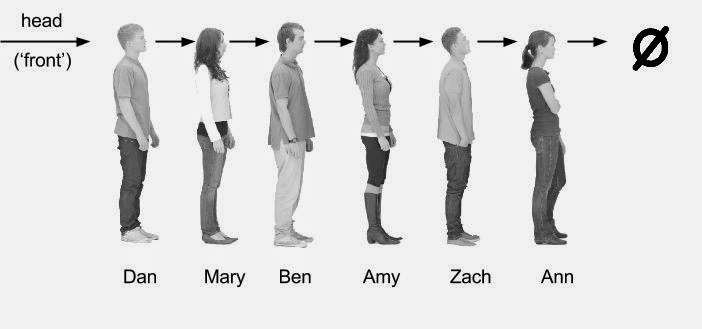
\includegraphics[height=3.3cm, width=7cm]{figs/fig_listas/ilustra_lista.jpg}
%\hspace{+0.25cm}
%\scriptsize\textcolor{red}{[Tizio, Caio et al., Nature (2006)]}
\end{column}
\end{columns}


\end{frame}
%----------------------------------------------------------------------------------------------------------
\begin{frame}

\begin{block}{ \textcolor{red}{Atenção:} }

\begin{itemize}
  \item \textcolor{red}{Duas partes este capítulo}
  \item   Listas com um vetor de tamanho fixo internamente
  \item  Listas estruturadas em nós alocados dinamicamente
  \item  Conceitualmente, equivalentes!
  \item  Implementações e exemplos aqui discutidas: alocação dinâmica!
  \item  Aqui justifica-se o estudo extensivo de 
  ponteiros no início do curso
  \item  A terminologia aqui adotada é proveniente de vários livros e do professor! 
\end{itemize}

\end{block}

\end{frame}
%----------------------------------------------------------------------------------------------------------


%----------------------------------------------------------------------------------------------------------

\subsection{Listas -- Tamanho Limitado}
  \begin{frame}{Introdução}    
		\begin{itemize}
			\item Uma seqüência de nós ou elementos dispostos em uma ordem estritamente linear.
			\item Cada elemento da lista é acessível um após o outro, em ordem.
			\item Pode ser implementada de várias maneiras			
				\begin{enumerate}
					\item Em um vetor
					\item Em uma estrutura que tem um vetor de tamanho fixo e uma 
					variável para armazenar o tamanho da lista
					\item Conjunto de nós criados e ligados dinâmicamente (abordagem aqui adotada nos códigos apresentados)
					\pause
					\item As duas implementações iniciais são exercícios de disciplinas anteriores.
				\end{enumerate}
		\end{itemize}
  \end{frame}

%----------------------------------------------------------------------------------------------------------
  \begin{frame}{Motivação}    
	\begin{enumerate}
	\item Talvez a estrutura de dados mais importante
	\item Generaliza Pilhas e Filas
	\item Utilizada em várias outras estruturas como grafos e árvores
	\pause
	\item Os exemplos em código apresentados, utilizam extensivamente 
	endereçamentos de memória (ponteiros e ponteiros para ponteiros) e alocações dinãmicas
	de memória
	\item Contudo, para fins conceitual usaremos uma lista {\em rígida} nestes slides -- 1a. parte
	\end{enumerate}
	
  \end{frame}
%----------------------------------------------------------------------------------------------------------
\begin{frame}{Aplicações}    
	\begin{enumerate}
	\item Uso em outros algoritmos e estrutura de dados como árvores e grafos
	\pause
	\item Conceitualmente, todo estudo aqui feito é aplicado
	aos outros paradigmas de linguagens de programação 
	\end{enumerate}
	
  \end{frame}
%----------------------------------------------------------------------------------------------------------

\begin{frame}
\frametitle{Exemplo de Uso}
\begin{figure}[!hb]
	\centering
		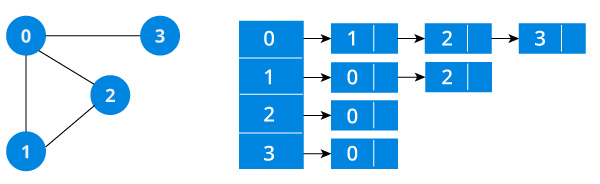
\includegraphics[height=0.30\paperheight, width=0.55\paperwidth]{figs/fig_listas/lista_matriz_adjacencia}			
			\caption{Uso de lista para representar matriz de adjacência}	
%%				\label{fig:lista-linear-repre}
			\end{figure} 

  \end{frame}
%----------------------------------------------------------------------------------------------------------



%----------------------------------------------------------------------------------------------------------  
\begin{frame}{Definição}
     \begin{block}{Definição}
     \begin{itemize}
       \item Um conjunto de nós, $x_1, x_2, x_3, \cdots, x_n$, organizados estruturalmente de forma a refletir as posições relativas dos mesmos. 
       \item  Se $n > 0$, então $x_1$ é o primeiro nó.
      \item Seja $L$ uma lista de $n$ nós, e $x_k$ um nó $\in$ L e $k$ a posição do nó em $L$. 
      \item  Então, $x_k$ é precedido pelo nó $x_{k-1}$ e seguido pelo nó $x_{k+1}$. 
      \item  O último nó de $L$ é $x_{n-1}$. Quando $n = 0$, dizemos que a lista está vazia.
       \end{itemize}
     \end{block}     
\end{frame}
%----------------------------------------------------------------------------------------------------------



%----------------------------------------------------------------------------------------------------------
\begin{frame}{Representação}
\begin{itemize}
	\item Os nós de uma lista são armazenados em {\it endereços contínuos} (apenas os endereços)
	\item A relação de ordem é representada pelo fato de que se o endereço do 
	nó $x_i$ é conhecido, então o endereço do nó $x_{i+1}$ também pode ser determinado. 	
	\item A Figura \ref{fig:lista-linear-repre} apresenta a representação de
	 uma lista linear de $n$ nós, com endereços representados por $k$
\end{itemize}

\begin{figure}[hb]
	\centering
		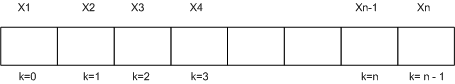
\includegraphics[width=.6\textwidth]{figs/fig_listas/lista-linear.png}			
			\caption{Exemplo de representação de lista -- usando um vetor}	
				\label{fig:lista-linear-repre}
			\end{figure} 
\end{frame}
%----------------------------------------------------------------------------------------------------------
\begin{frame}[fragile,c]{Representação como um Vetor de Inteiros}
\begin{itemize}
	\item Para exemplificar a implementações em C, vamos considerar que 
	o conteúdo armazenado na lista é do tipo inteiro (nos códigos são {\it strings}).
	\item A estrutura da lista possui a seguinte representação:	
\end{itemize}
\begin{lstlisting}[language=C]
  struct lista{
    int cursor;
    int elemento[N];
  }
  typedef struct lista Lista;
\end{lstlisting}

\begin{itemize}
	\item Trata-se de uma estrutura heterogênea constituída de membros distintos entre si. 
	\item Os membros são as variáveis \alert{\textit{cursor}}, a qual  armazena a  	quantidade de elementos da lista, e o vetor \alert{\textit{elemento}} de inteiros 	que armazena os nós da lista.
	\item Até o momento uma alocação estática -- lembra filas e pilhas
\end{itemize}
\end{frame}
%----------------------------------------------------------------------------------------------------------

\begin{frame}[fragile,c]{Representação Estática -- Tamanho Fixo}
\begin{itemize}

 \item Para atribuirmos um valor a algum membro da lista devemos utilizar a seguinte notação:

\small	
\begin{lstlisting}[language=C]
Lista->elemento[0] = 1 //atribui o valor 1 ao primeiro elemento da lista.
Lista->elemento[n-1] = 4 //atribui o valor 4 ao ultimo elemento da lista.
\end{lstlisting}
\end{itemize}
\end{frame}  
%----------------------------------------------------------------------------------------------------------

\begin{frame}{Operações Primitivas}
  \begin{itemize}
	  \item As operações básicas que devem ser implementadas em uma estrutura do tipo Lista são:		
  \end{itemize}
  \begin{table}[!htpb]
	\centering
    \begin{tabular}{l|l}
	 \hline \hline 
	 \textbf{Operação} & \textbf{Descrição} \\
	\hline \hline \\
	criar() & cria uma lista vazia.\\
	 \hline inserir(l,e) & insere o elemento \textit{e} no final da lista \textit{l}.\\
	 \hline remover(l,e) & remove o elemento \textit{e} da lista \textit{l}.\\
	\hline imprimir(l) & imprime os elementos da lista \textit{l}.\\
	\hline pesquisar(l,e) & pesquisa o elemento \textit{e} na lista \textit{l}.\\
	\hline 	\hline 
	\end{tabular}
	\caption{Operações básicas da estrutura de dados lista.}
\end{table}
\end{frame}
%----------------------------------------------------------------------------------------------------------
 
\begin{frame}{Operações auxiliares}   
	\begin{itemize}
	\item Além das operações básicas, temos as operações ``\textit{auxiliares}''. São elas:
	\end{itemize}
	\begin{table}[!htpb]
	  \centering
	\begin{tabular}{l||l}
	    \hline \hline 
	 \textbf{Operação} & \textbf{Descrição} \\
	\hline \hline \\
	    \hline empty(l) & determina se a lista \textit{l} está ou não vazia.\\
	    \hline destroy(l) & libera o espaço ocupado na memória pela lista \textit{l}.\\
	    \hline \hline
	\end{tabular}
\caption{Operações auxiliares da estrutura de dados lista.}
\end{table}
 \end{frame}
 
%----------------------------------------------------------------------------------------------------------

\begin{frame}[fragile,plain]{Interface do Tipo Lista}
\footnotesize
\begin{lstlisting}[language=C]
/* Aloca dinamicamente a estrutura lista, inicializando 
 * seus campos e retorna seu ponteiro. A lista depois 
 * de criada terah tamanho igual a zero. Sem malloc ... ainda */
Lista* criar(void);

/* Insere o elemento e no final da lista l, desde que,
 * a lista nao esteja cheia ... dada a limitacao inicial */
void inserir(Lista* l, int e);

/* Remove o elemento e da lista l,
 * desde que a lista nao esteja vazia e o elemento
 * e esteja na lista. A funcao retorna 0 se o elemento 
 * nao for encontrado na lista ou 1 caso contrario. */
void remover(Lista* l, int e);

/* Pesquisa na lista l o elemento e. A funcao retorna 
 * o endereco(indice) do elemento se ele pertencer a lista
 * ou -1 caso contrario.*/
int pesquisar(Lista* l, int e);

/* Lista os elementos da lista l. */
void imprimir(Lista* l);
\end{lstlisting}
\end{frame}
%----------------------------------------------------------------------------------------------------------

\begin{frame}{Implementação das Listas de Tamanho Fixo}

A utilização de vetores para implementar a lista traz algumas vantagens como:	
  \begin{enumerate}
	\item Os elementos são armazenados em posições contíguas da memória
	\item Basta ver a estrutura, internamente é um vetor
	\item Economia de memória, pois os ponteiros para o próximo elemento da lista são explícitos
	\item Há um índice de acesso direto e o {\em cursor} para indicar o último elemento
\end{enumerate}

\end{frame}

%----------------------------------------------------------------------------------------------------------
\begin{frame}{Implementação das Listas de Tamanho Fixo}

No entanto, as desvantagens são:		
  \begin{enumerate}
\item Custo de inserir/remover elementos da lista 
\pause
\item Neste caso se refere ao deslocamento células a frente no caso de inserção
\pause
\item ou  deslocamento células para trás no caso de remoção
\pause
\item Finalmente: limitação da quantidade de elementos da lista
\item Este é ponto ... tamanho fixo!
\item Aqui, usamos alocação dinâmica, mas todos conceitos aqui são complementares
\end{enumerate}

\end{frame}
%----------------------------------------------------------------------------------------------------------

\begin{frame}[fragile,c]{Função de Criação}
	\begin{itemize}
	\item A função que cria uma lista, deve criar e retornar uma lista vazia;
	\item A função deve atribuir o valor zero ao tamanho da lista, ou seja, fazer $l->cursor = 0$, como podemos ver no código abaixo.
	\item A complexidade de tempo para criar a lista é constante, ou seja, $O(1)$.
	\end{itemize}
	
\begin{lstlisting}[language=C]
/*
 * Aloca dinamicamente a estrutura lista, inicializando seus
 * campos e retorna seu ponteiro. A lista depois de criada
 * terah tamanho igual a zero.
 */
Lista* criar(void){
  Lista* l = (Lista*) malloc(sizeof(Lista));
  l->cursor = 0;
  return l;
}
\end{lstlisting}
\end{frame}
%----------------------------------------------------------------------------------------------------------

\begin{frame}[fragile,c]{Função de Inserção}  
	\begin{itemize}
	\item A inserção de qualquer elemento ocorre no final da lista, desde que a lista não esteja cheia.
	\item Com isso, para inserir um elemento basta atribuirmos o valor ao elemento cujo índice é o valor referenciado pelo campo \textit{cursor}, e incrementar o valor do cursor, ou seja fazer 
	\texttt{l->elemento[l->cursor++] = valor}, como podemos verificar no código abaixo, a uma complexidade de tempo constante, $O(1)$.
	\end{itemize}

\footnotesize
\begin{lstlisting}[language=C]
/*
 * Insere o elemento e no final da lista l, desde que,
 * a lista nao esteja cheia.
 */
void inserir(Lista* l, int e){
  if (l == NULL || l->cursor == N){
    printf("Error. A lista esta cheia\n");
  }else{
    l->elemento[l->cursor++] = e;
  }
}
\end{lstlisting}	
\end{frame}
%----------------------------------------------------------------------------------------------------------

\begin{frame}[fragile,c]{Função de Remoção} 
	\begin{itemize}
		\item Para remover um elemento da lista, primeiro precisamos verificar se ele está na lista, para assim removê-lo, e deslocar os seus sucessores, quando o elemento removido não for o último.
		\item A complexidade de tempo da função de remoção é $O(n)$, pois é necessário movimentar os $n$ elementos para remover um elemento e ajustar a lista.
	\end{itemize}
	
\footnotesize
\begin{lstlisting}[language=C]
/* remove um elemento da lista */
void remover(Lista* l, int e){     
  int i, d = pesquisar(l,e);
  if (d != -1){
    for(i = d; i < l->cursor; i++)
    {
      l->elemento[i] = l->elemento[i + 1];
    }
    l->cursor--;
  }  
}
\end{lstlisting}	
\end{frame} 
%----------------------------------------------------------------------------------------------------------

\begin{frame}[fragile]{Função de Pesquisa} 
   \begin{itemize}
	\item Para pesquisar um elemento qualquer na lista é necessário compará-lo com os elementos existentes, utilizando alguns dos algoritmos de busca conhecidos;
	\item A complexidade de tempo dessa função depende do algoritmo de busca implementado. Se utilizarmos a busca seqüencial, a complexidade da função será $O(n)$. No entanto, é possível baixá-lo para $O(n\log n)$.
 \end{itemize}

\footnotesize
\begin{lstlisting}[language=C]
int pesquisar(Lista* l, int e){
  if (l == NULL)
    return;
  
  int i = 0;
  while (i <= l->cursor && l->elemento[i] != e)
    i++;
        
  return i > l->cursor ? -1 : i;
}
\end{lstlisting}
\end{frame}
%----------------------------------------------------------------------------------------------------------

\begin{frame}[fragile]{Função de Impressão}

\begin{itemize}

\item A impressão da lista ocorre através da apresentação de todos os elementos compreendidos entre o intervalo: 
  $[0 .. l->cursor]$.

\item A complexidade de tempo da função de impressão é $O(n)$, pois no 
  pior caso, quando lista estiver cheia, é necessário percorrer 
  os $n$ elementos da lista.
\end{itemize}
	
\begin{lstlisting}[language=C]
/* Apresenta os elementos da lista l. */
void imprimir(Lista* l){
 int i;
 for(i = 0; i < l->cursor; i++)
   printf("%d ", l->elemento[i]);
 printf("\n");  
}
\end{lstlisting}	
\end{frame}
%----------------------------------------------------------------------------------------------------------

\begin{frame}[fragile,c]{Exemplo de Uso da Lista}

\begin{lstlisting}[language=C]
\#include <stdio.h>
\#include "list.h"
int main(void)
{
    Lista* l = criar();
    int i, j = 4;
    
    /* Inserir 5 elementos na lista */
    for (i = 0; i < 5; i++)
      inserir(l,j * i);
    
    /* Apresenta os elementos inseridos na lista*/    
    imprimir(l);
    /* Remove o segundo elemento da lista*/
    remover(l,j);
    /* Apresenta os elementos da lista */    
    imprimir(l);        
}
\end{lstlisting}

\end{frame} 

%----------------------------------------------------------------------------------------------------------

\subsection{Listas -- Tamanho Ilimitado}
\begin{frame}%%[allowframebreaks=0.98]
\frametitle{Listas Dinamicamente Encadeadas -- LE}


\begin{block}{\textcolor{red}{Atenção:}}
\begin{itemize}
  \item Esta é a 2a. parte do capítulo
  \item Os conceitos vistos com listas de \textit{arrays}, agora com
  nós alocados dinamicamente
  \item Acompanhe os exemplos do repositório da disciplina
  \item Basicamente os métodos são os mesmos visto para lista com \textit{arrays}
\end{itemize}
\end{block}

\end{frame} 


%----------------------------------------------------------------------------------------------------------

\begin{frame}
\frametitle{Listas Encadeadas  (ora Listas \textit{Ilimitadas})}

\begin{block}{Complemento}

\begin{itemize}
  \item Nesta parte vamos discutir as listas \textit{ilimitadas}
  \item Crescem ou não dinâmicamente de acordo com a disponibilidade de memória
  \item O usuário controla a memória etc
  \item Todos conceitos vistos anteriormente, são aqui preservados
  \item .... 
\end{itemize}

\end{block}

\end{frame} 

%---------------------------------------------------------------------------------------------------------
%[allowframebreaks=0.9]


\begin{frame}%%[allowframebreaks=0.98]
\frametitle{Estrutura clássica  da implementação dessas listas}

\begin{figure}[!ht]
	\centering
	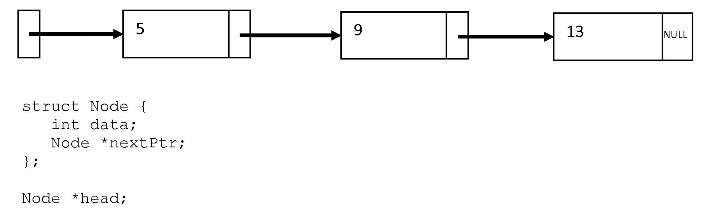
\includegraphics[height=0.550\paperheight, width=0.85\paperwidth]{figs/fig_listas/lista_SE_struct}
\caption{Lista Simplesmente Encadeada -- LSE ou LE}
	\end{figure} 
	
\begin{center}
	\textcolor{red}{Conceitualmente, nada foi modificada em relação ao que se tinha anteriormente!}
	\end{center}

\end{frame} 

%%%%
\begin{frame}%%[allowframebreaks=0.98]
\frametitle{\textit{Espalhadas} pela memória principal ... não contíguas!}

\begin{figure}[!ht]
	\centering
	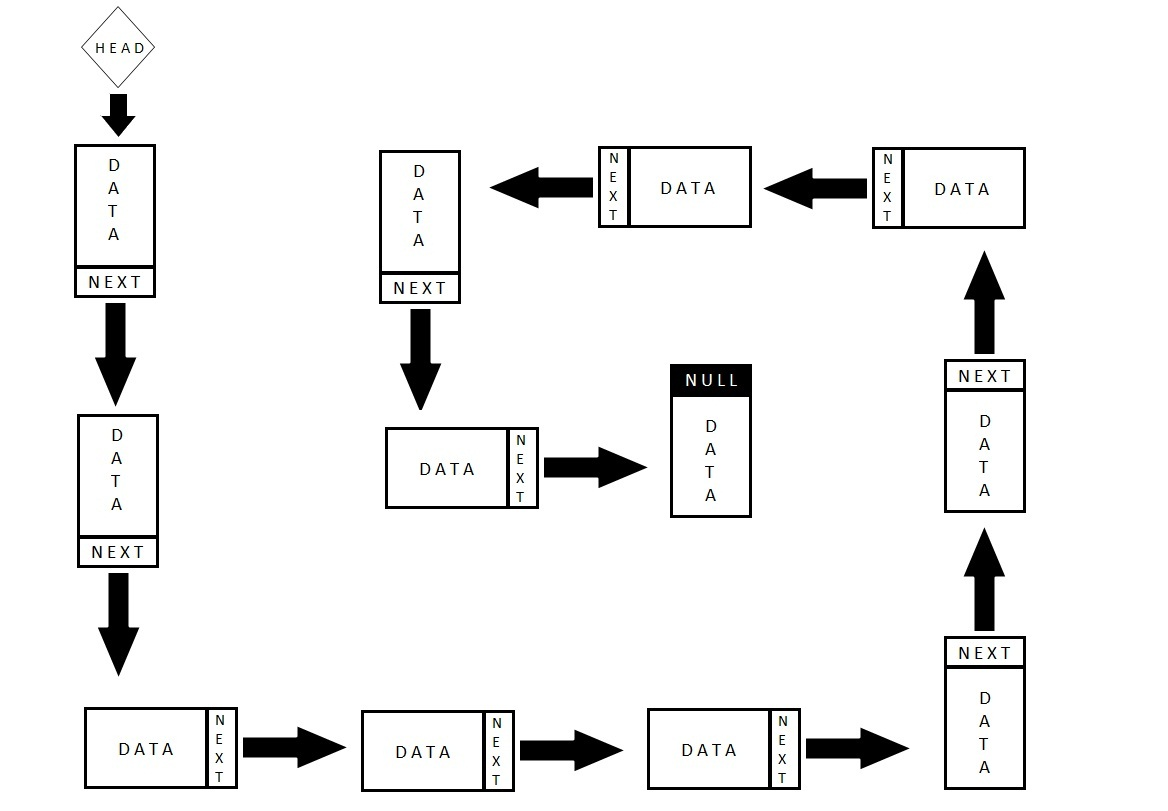
\includegraphics[height=0.550\paperheight, width=0.85\paperwidth]{figs/fig_listas/lista_encadeada02}
\caption{Lista Simplesmente Encadeada -- LSE}
	\end{figure} 

\end{frame} 

%----------------------------------------------------------------------------------------------------------
%----------------------------------------------------------------------------------------------------------

\begin{frame}%[allowframebreaks=0.8]
\frametitle{\textit{Truques}  destas Implementações de Listas}


\begin{block}{\textcolor{red}{Observações:}}

\begin{itemize}
  \item Ao contrário do que foi visto, estas estruturas são alocadas
  dinamicamente na MP;
  \item Idem quanto as remoções e a sua liberação de área;
  \item O ponto é que facilmente pode se perder o ponteiro de início de lista
  se o mesmo entrar no cálculo ou numa operação de lista;
  \item Logo, vamos passar apenas o seu endereço afim de preservá-lo na função   principal
    
\end{itemize}
\end{block}

\end{frame} 
%----------------------------------------------------------------------------------------------------------

\begin{frame}%[allowframebreaks=0.8]
\frametitle{\textit{Truques}  destas Implementações de Listas}

\begin{block}{\textcolor{red}{Observações:}}

\begin{itemize}
   \item Uma proteção (\textit{blindagem}) deste ponteiro cabeça de lista
   \item Ou seja, passando apenas o seu endereço para as funções, estas terão que receber
   como um ponteiro de ponteiro!
   \item Sim, pois virá o endereço de um ponteiro que tem o início de lista, logo,
 uma estrutura de nó com um   ponteiro de ponteiro é agora interessante.
 \item Veja as implementações  e as estude com cuidado!
 
 \item Faça um desenho de tudo que está escrito ... vais precisar!
    
\end{itemize}
\end{block}

\end{frame} 

%----------------------------------------------------------------------------------------------------------

\begin{frame}%%[allowframebreaks=0.98]
\frametitle{Complexidade de Implementações de Listas}

\begin{figure}[!ht]
	\centering
	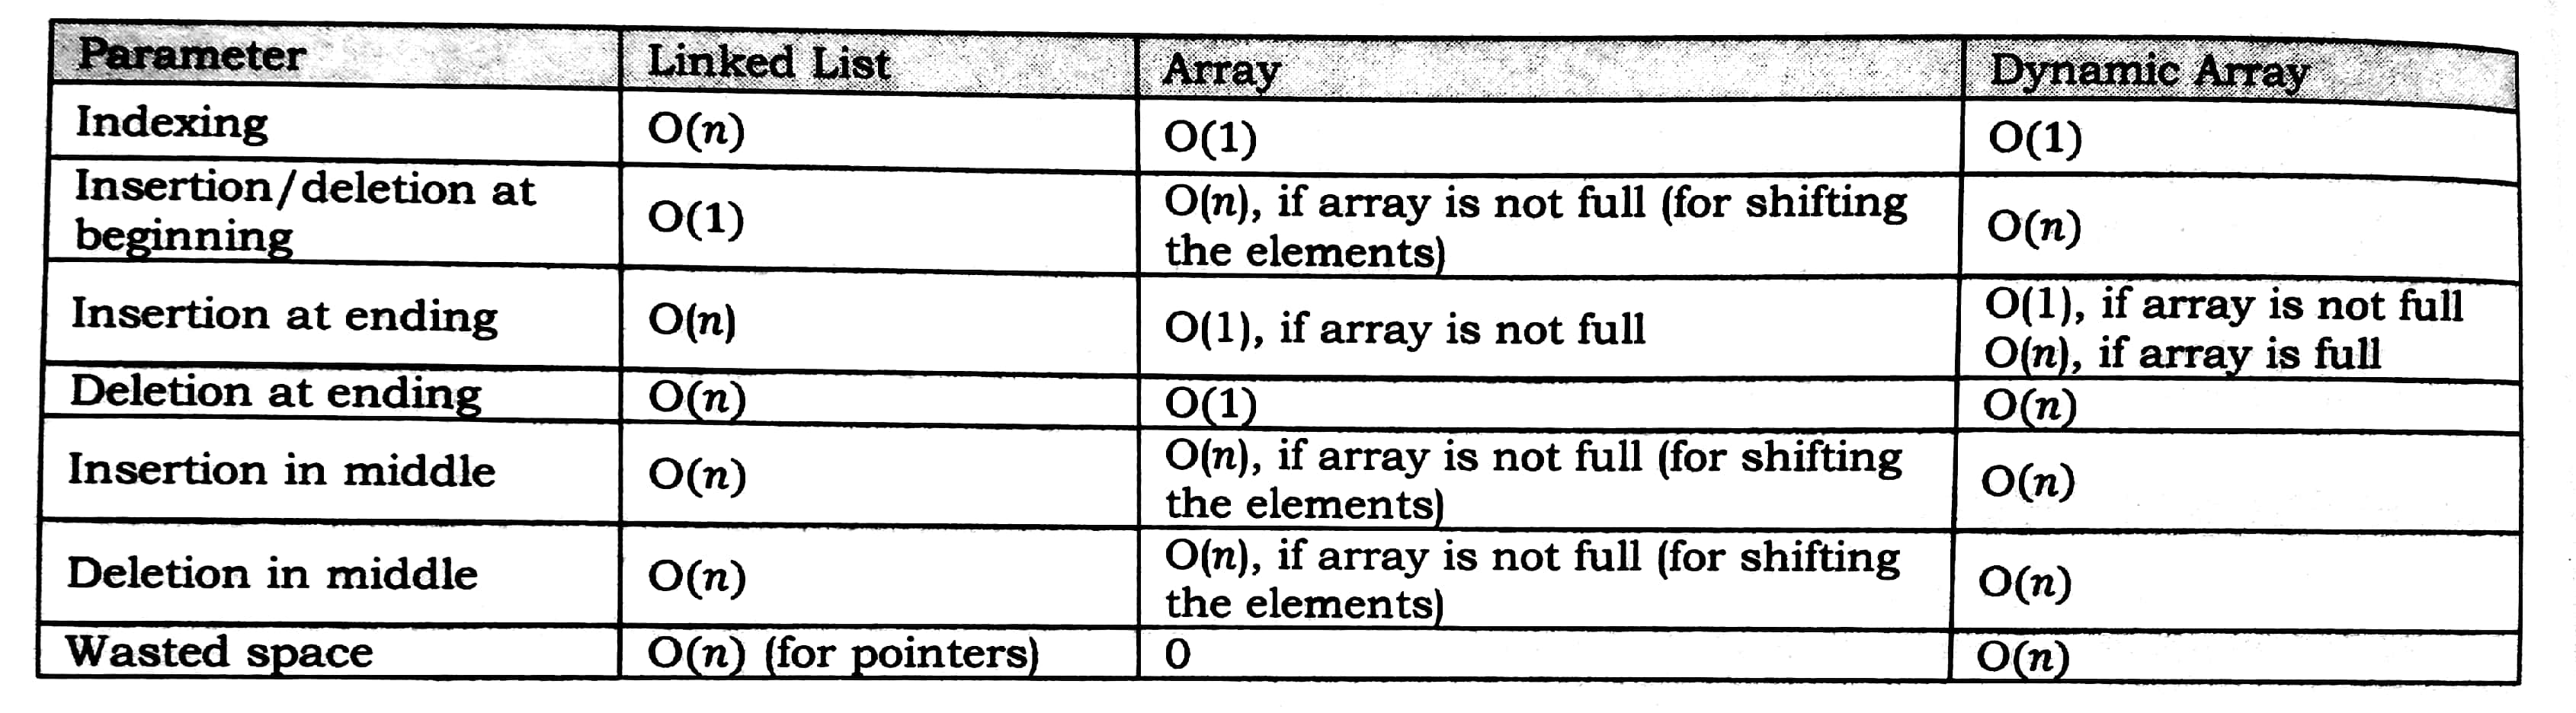
\includegraphics[height=0.560\paperheight, width=0.8\paperwidth]{figs/fig_listas/compara_implementacao_listas}
%%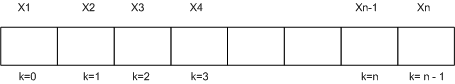
\includegraphics[height=0.50\paperheight, width=0.5\paperwidth]{figs/fig_listas/lista-linear}
\caption{Comparativo da complexidade quanto as implementações}
	\end{figure} 

\end{frame} 

%----------------------------------------------------------------------------------------------------------
%%[allowframebreaks=0.98]
\begin{frame}
\frametitle{Comparativo de Implementações de Listas --
\textit{Vetores} (dinâmicos e estáticos) $\times$ Nós Encadeados}

\begin{block}{Vantagens dos Vetores (ou \textit{Arrays}):}
\begin{itemize}
  \item Simples e fácil de usar
  \item Tempo de acesso constante, pois há um índice para acesso
  de seus elementos
  \item Se o \textit{arrays} for dinâmico, \textit{malloc} e \textit{realloc}, temos crescimento e encolhimentos adaptativos. Se e somente se forem dinâmicos!
\end{itemize}
\end{block}

\begin{block}{Desvantagens dos Vetores (ou \textit{Arrays}):}
\begin{itemize}
  \item Pré-aloca uma quantidade e permanece fixa até o final
  \item Desperdícios quando há células não utilizadas
  \item Complexo quanto a movimentações de células ou blocos (muitas células sendo inseridas ou excluídas simultaneamente $\approx $ operação em \textit{bloco})
\end{itemize}

\end{block}

\end{frame} 


%----------------------------------------------------------------------------------------------------------
%%[allowframebreaks=0.98]
\begin{frame}
\frametitle{Comparativo de Implementações de Listas --
\textit{Vetores} (dinâmicos e estáticos) $\times$ Nós Encadeados}

\begin{block}{Vantagens das listas:}
\begin{itemize}
  \item Crescem em tempo constante
  \item Operações como criar, destruir, tomam tempo constante, outras operações $O(n)$, ver tabela
  \item Não há desperdícios de memória: $alocou = usou$
\end{itemize}
\end{block}


\begin{block}{Desvantagens das listas:}
\begin{itemize}
  \item Principal problema é o tempo de acesso as células: num vetor $O(1)$ e nas listas $O(n)$
  \item Outro problema são os espaços contíguos: num vetor, quando alocado pode ir para uma memória \textit{cache}, e se beneficiar de mecanismos de \textit{caching} de CPUs e SOs modernos
  \item Finalmente, algum atraso em operações mais complexas, tal 
  como alocar um \texttt{NULL} no último ponteiro da lista
\end{itemize}

\end{block}

\end{frame} 

%----------------------------------------------------------------------------------------------------------

\begin{frame}%%[allowframebreaks=0.98]

\begin{center}
{\huge Implementações de Alguns Métodos}
\end{center}
\end{frame} 


%----------------------------------------------------------------------------------------------------------

\begin{frame}%%[allowframebreaks=0.98]
\frametitle{Incluindo um nó no início da lista}
\begin{figure}[!ht]
	\centering
	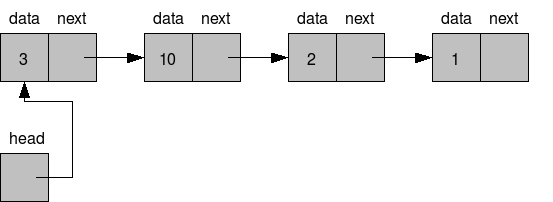
\includegraphics[height=0.30\paperheight, width=0.5\paperwidth]{figs/fig_listas/lista_encadeada01}
	\end{figure} 


\begin{figure}[!hb]
	\centering
		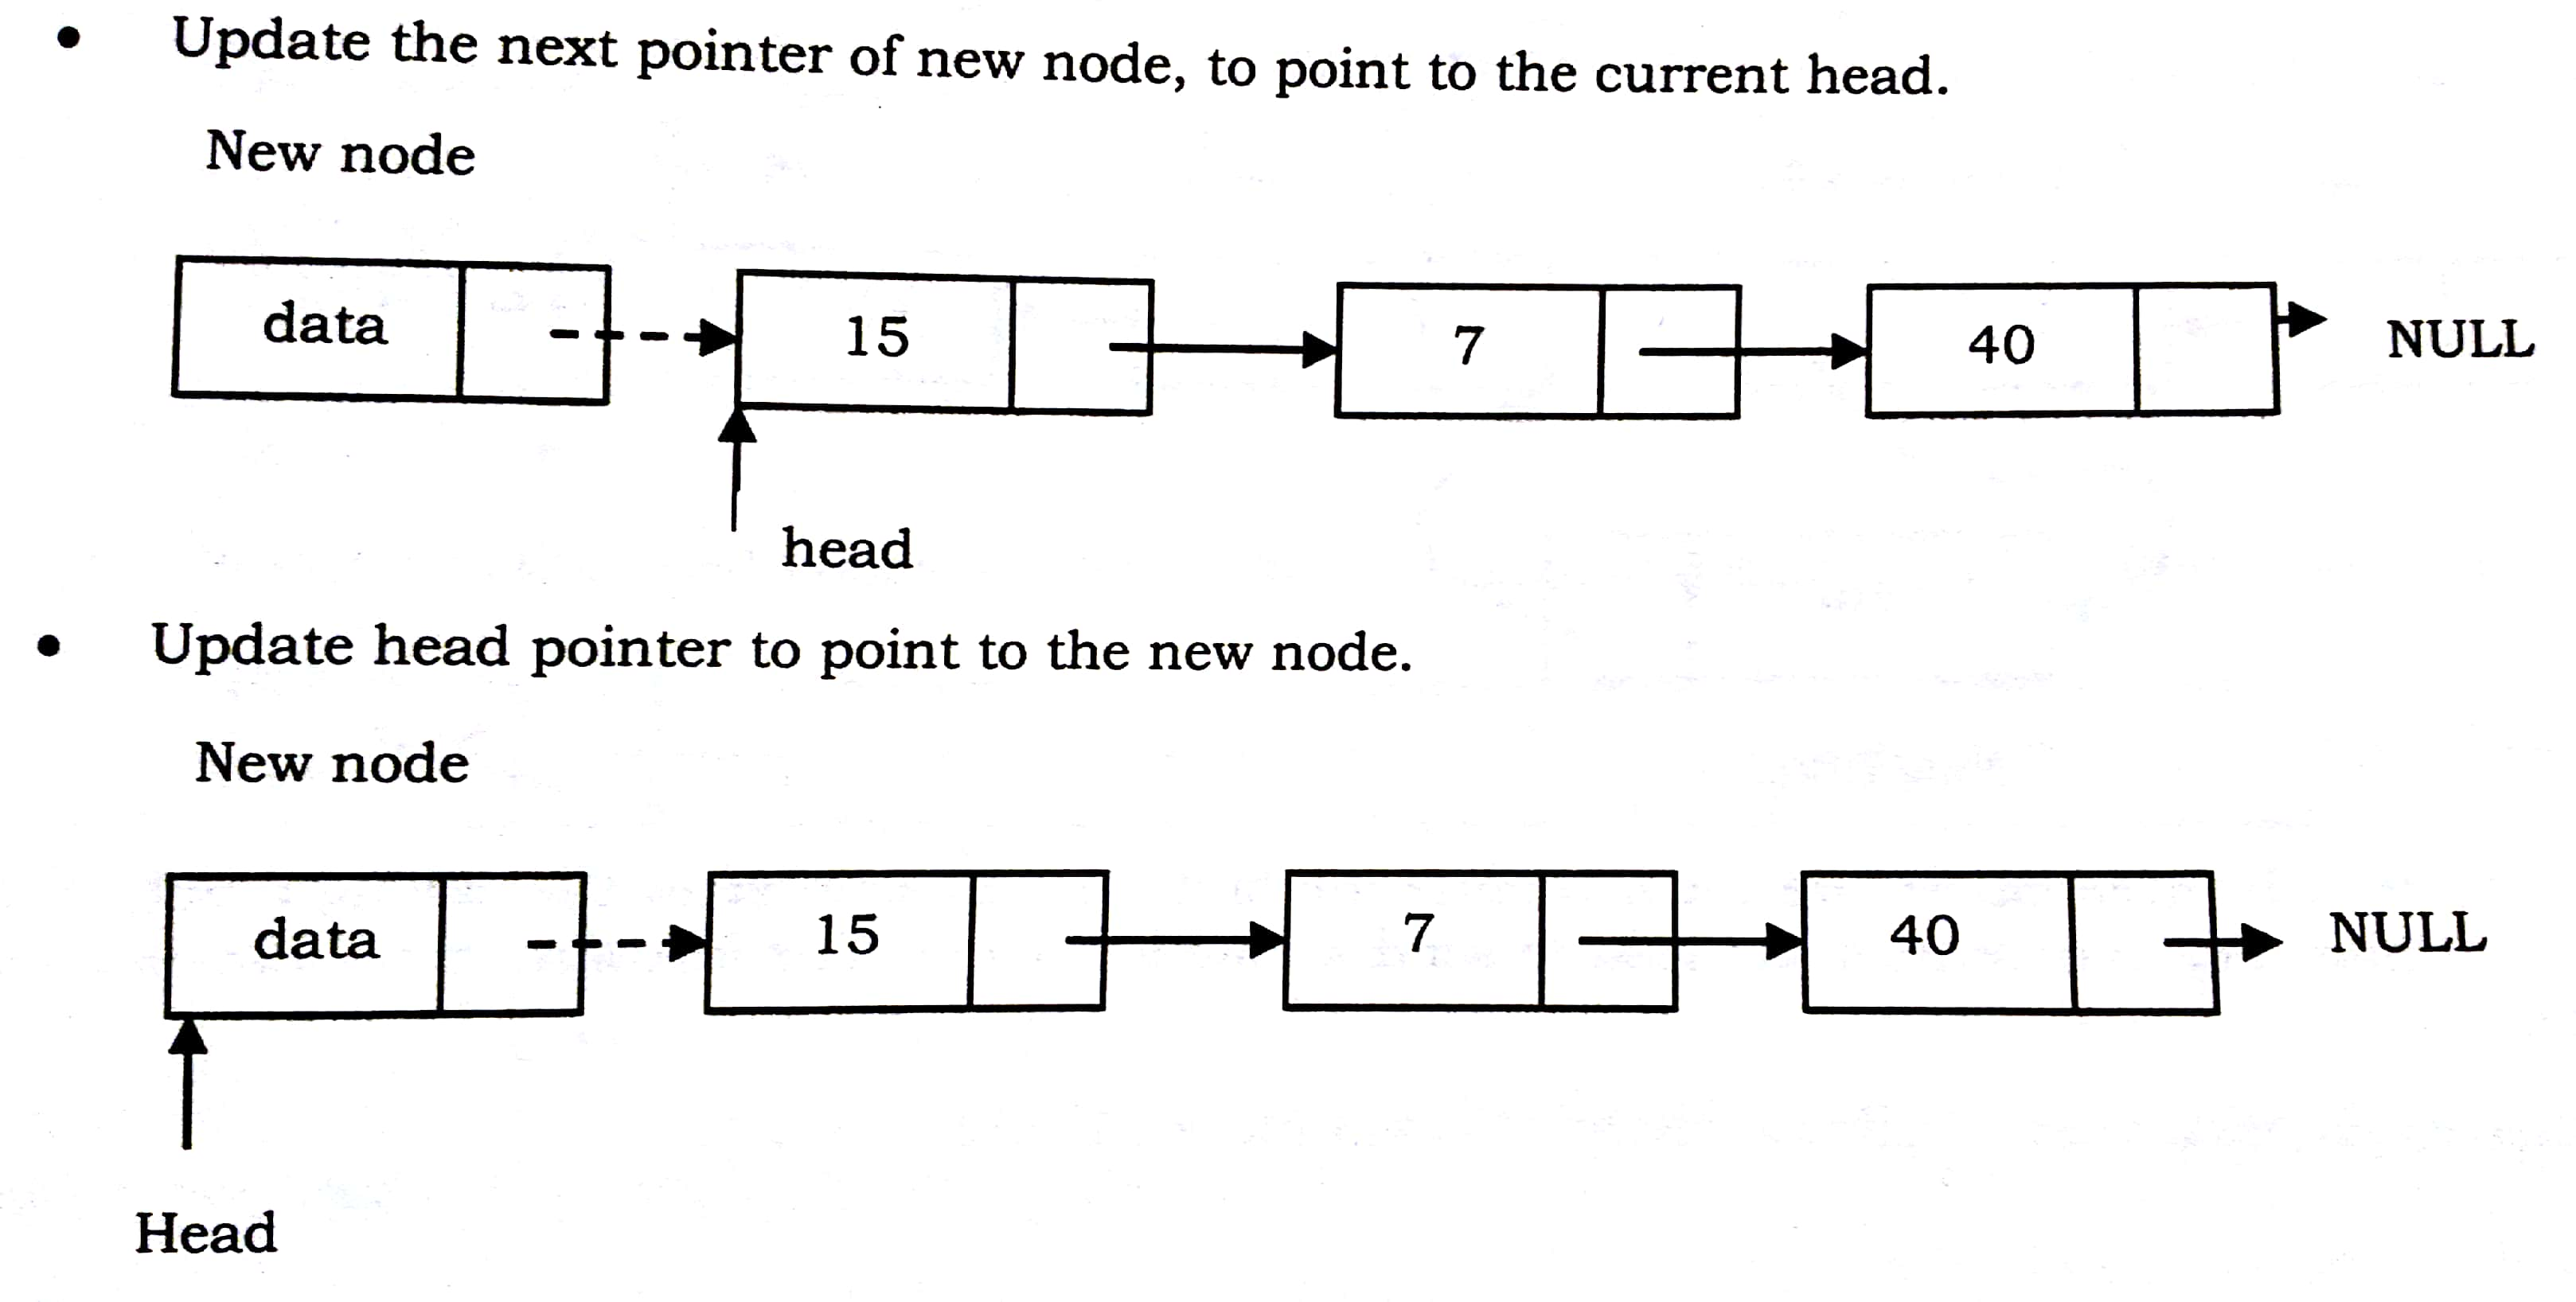
\includegraphics[height=0.50\paperheight, width=0.5\paperwidth]{figs/fig_listas/insere_inicio}			
			\caption{Incluir um nó no início da lista}	
%%				\label{fig:lista-linear-repre}
			\end{figure} 


\end{frame} 
%----------------------------------------------------------------------------------------------------------
%[allowframebreaks=0.9]

\begin{frame}%%%[allowframebreaks=0.98]

\frametitle{Incluindo um nó numa posição da  lista}

\begin{figure}[!hb]
	\centering
%%		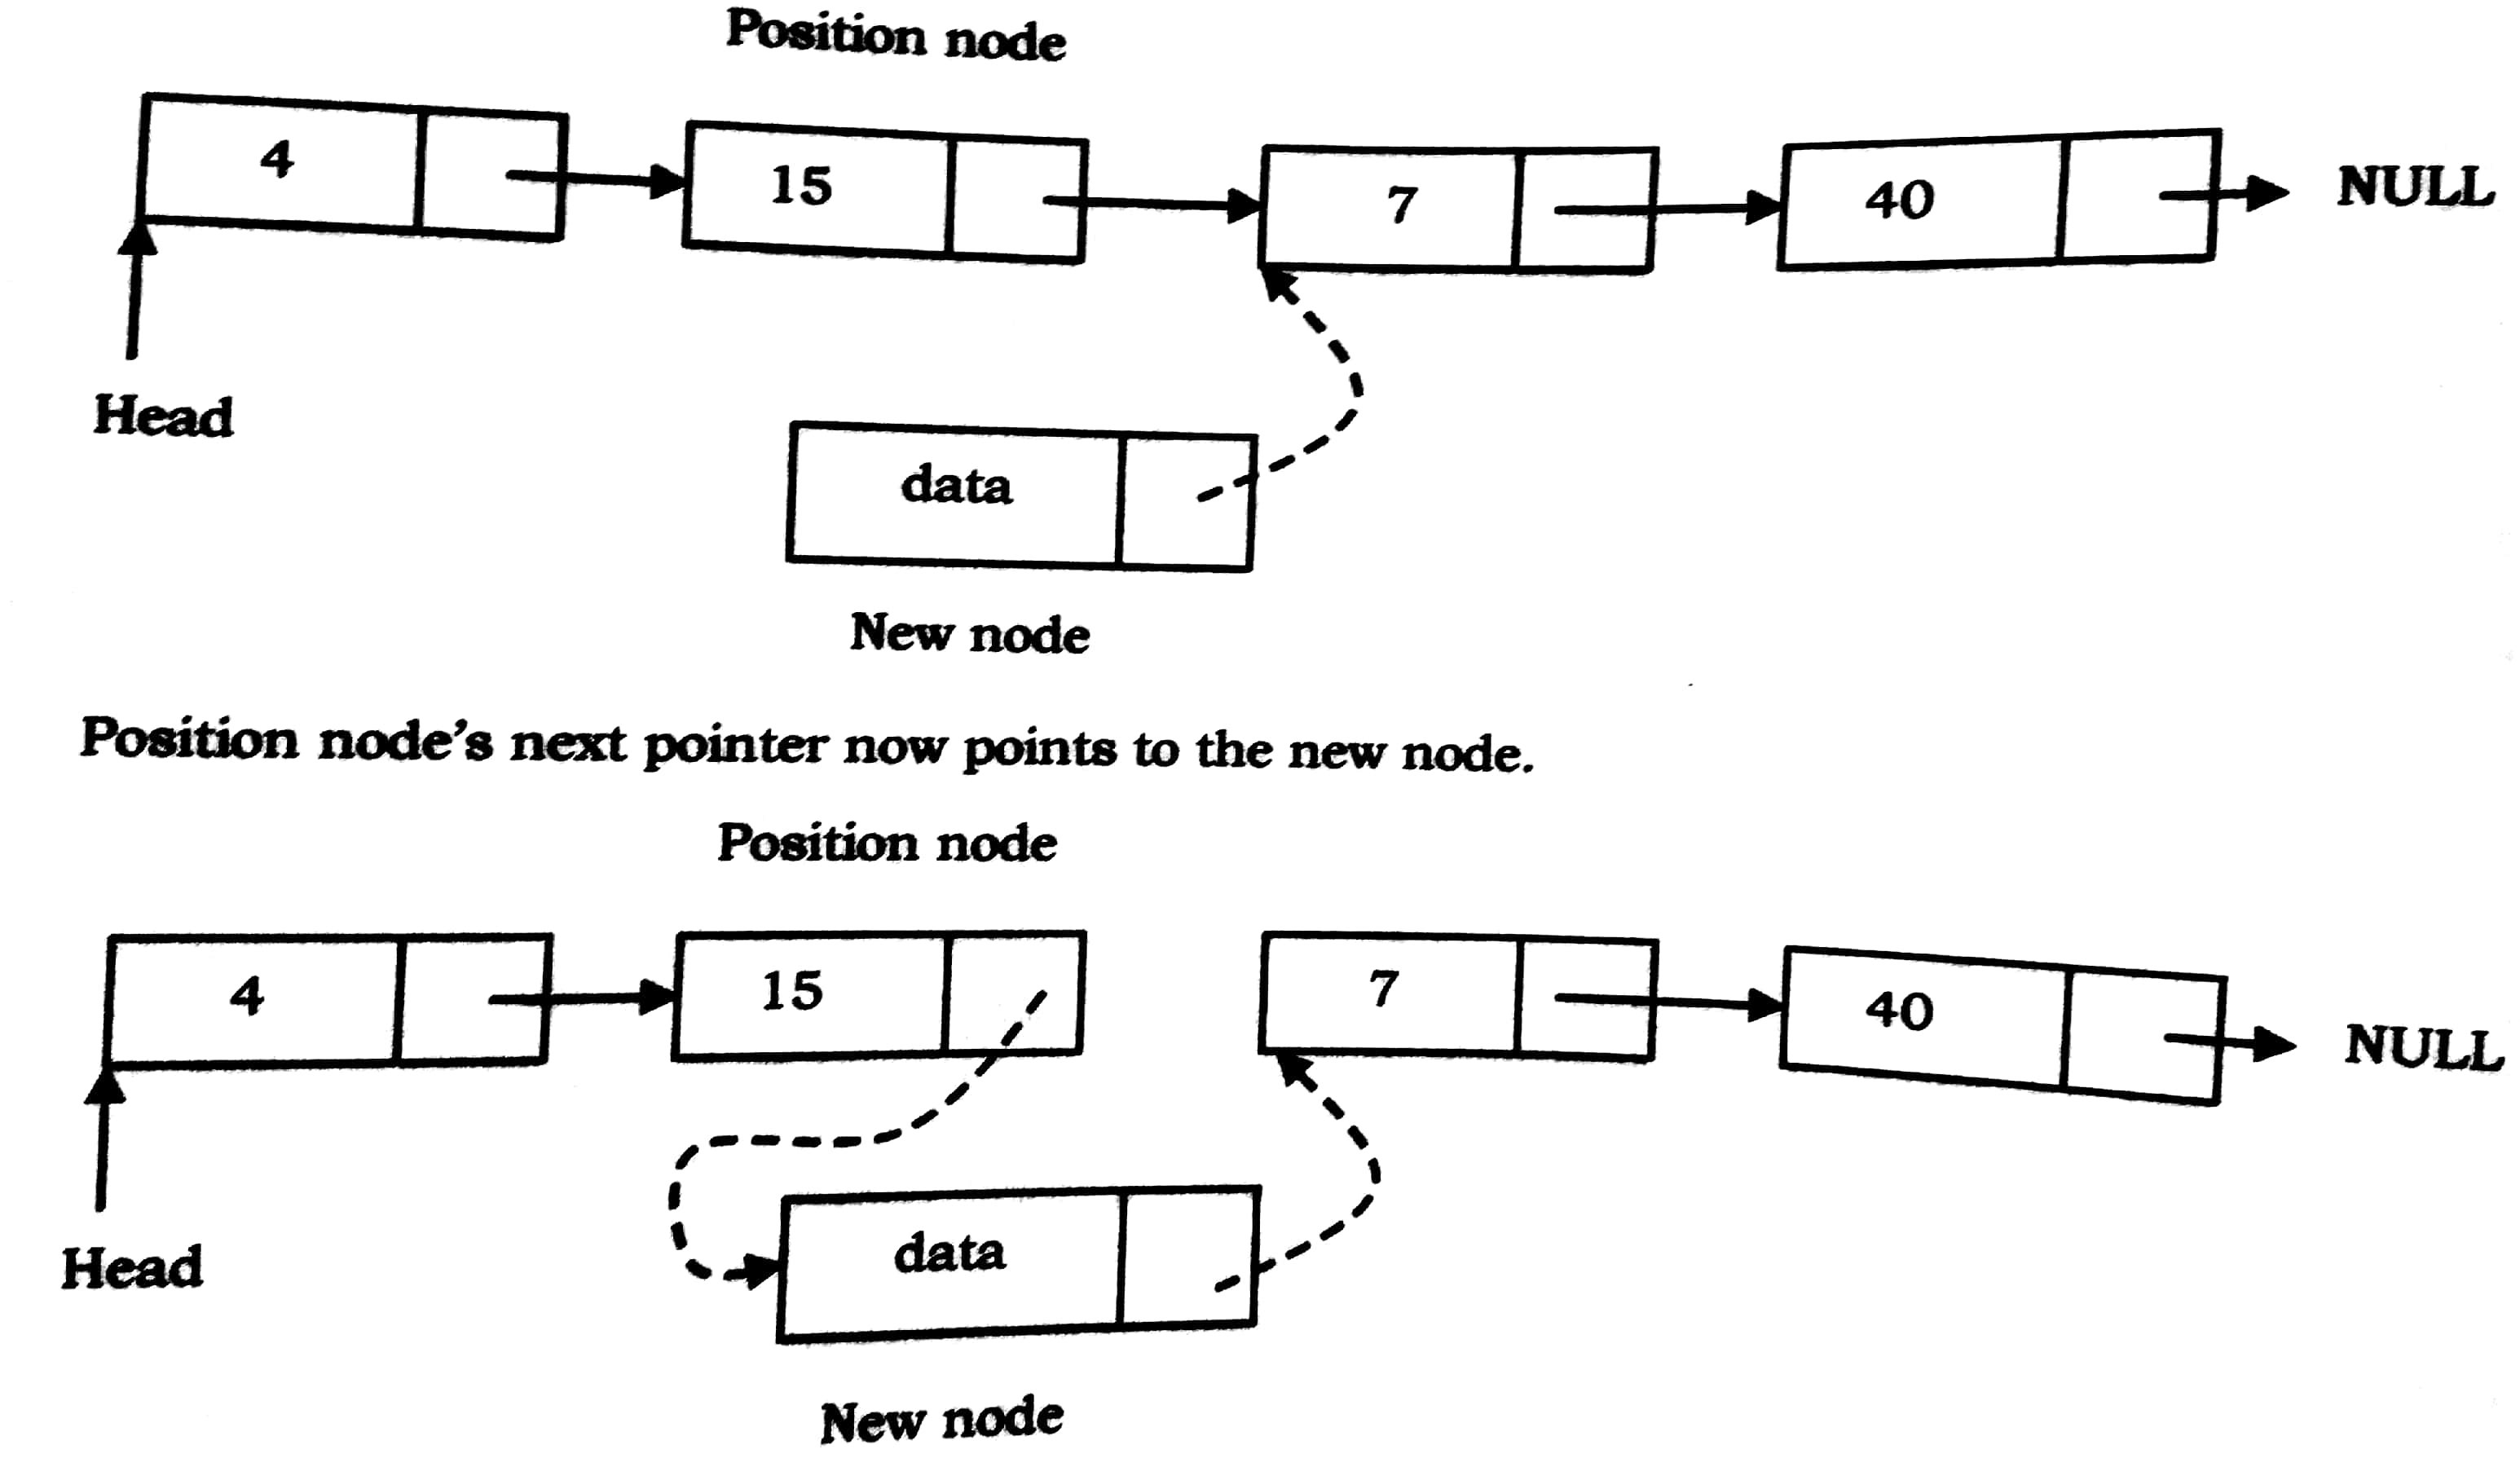
\includegraphics[scale=0.1]{figs/fig_listas/insere_posicao}
	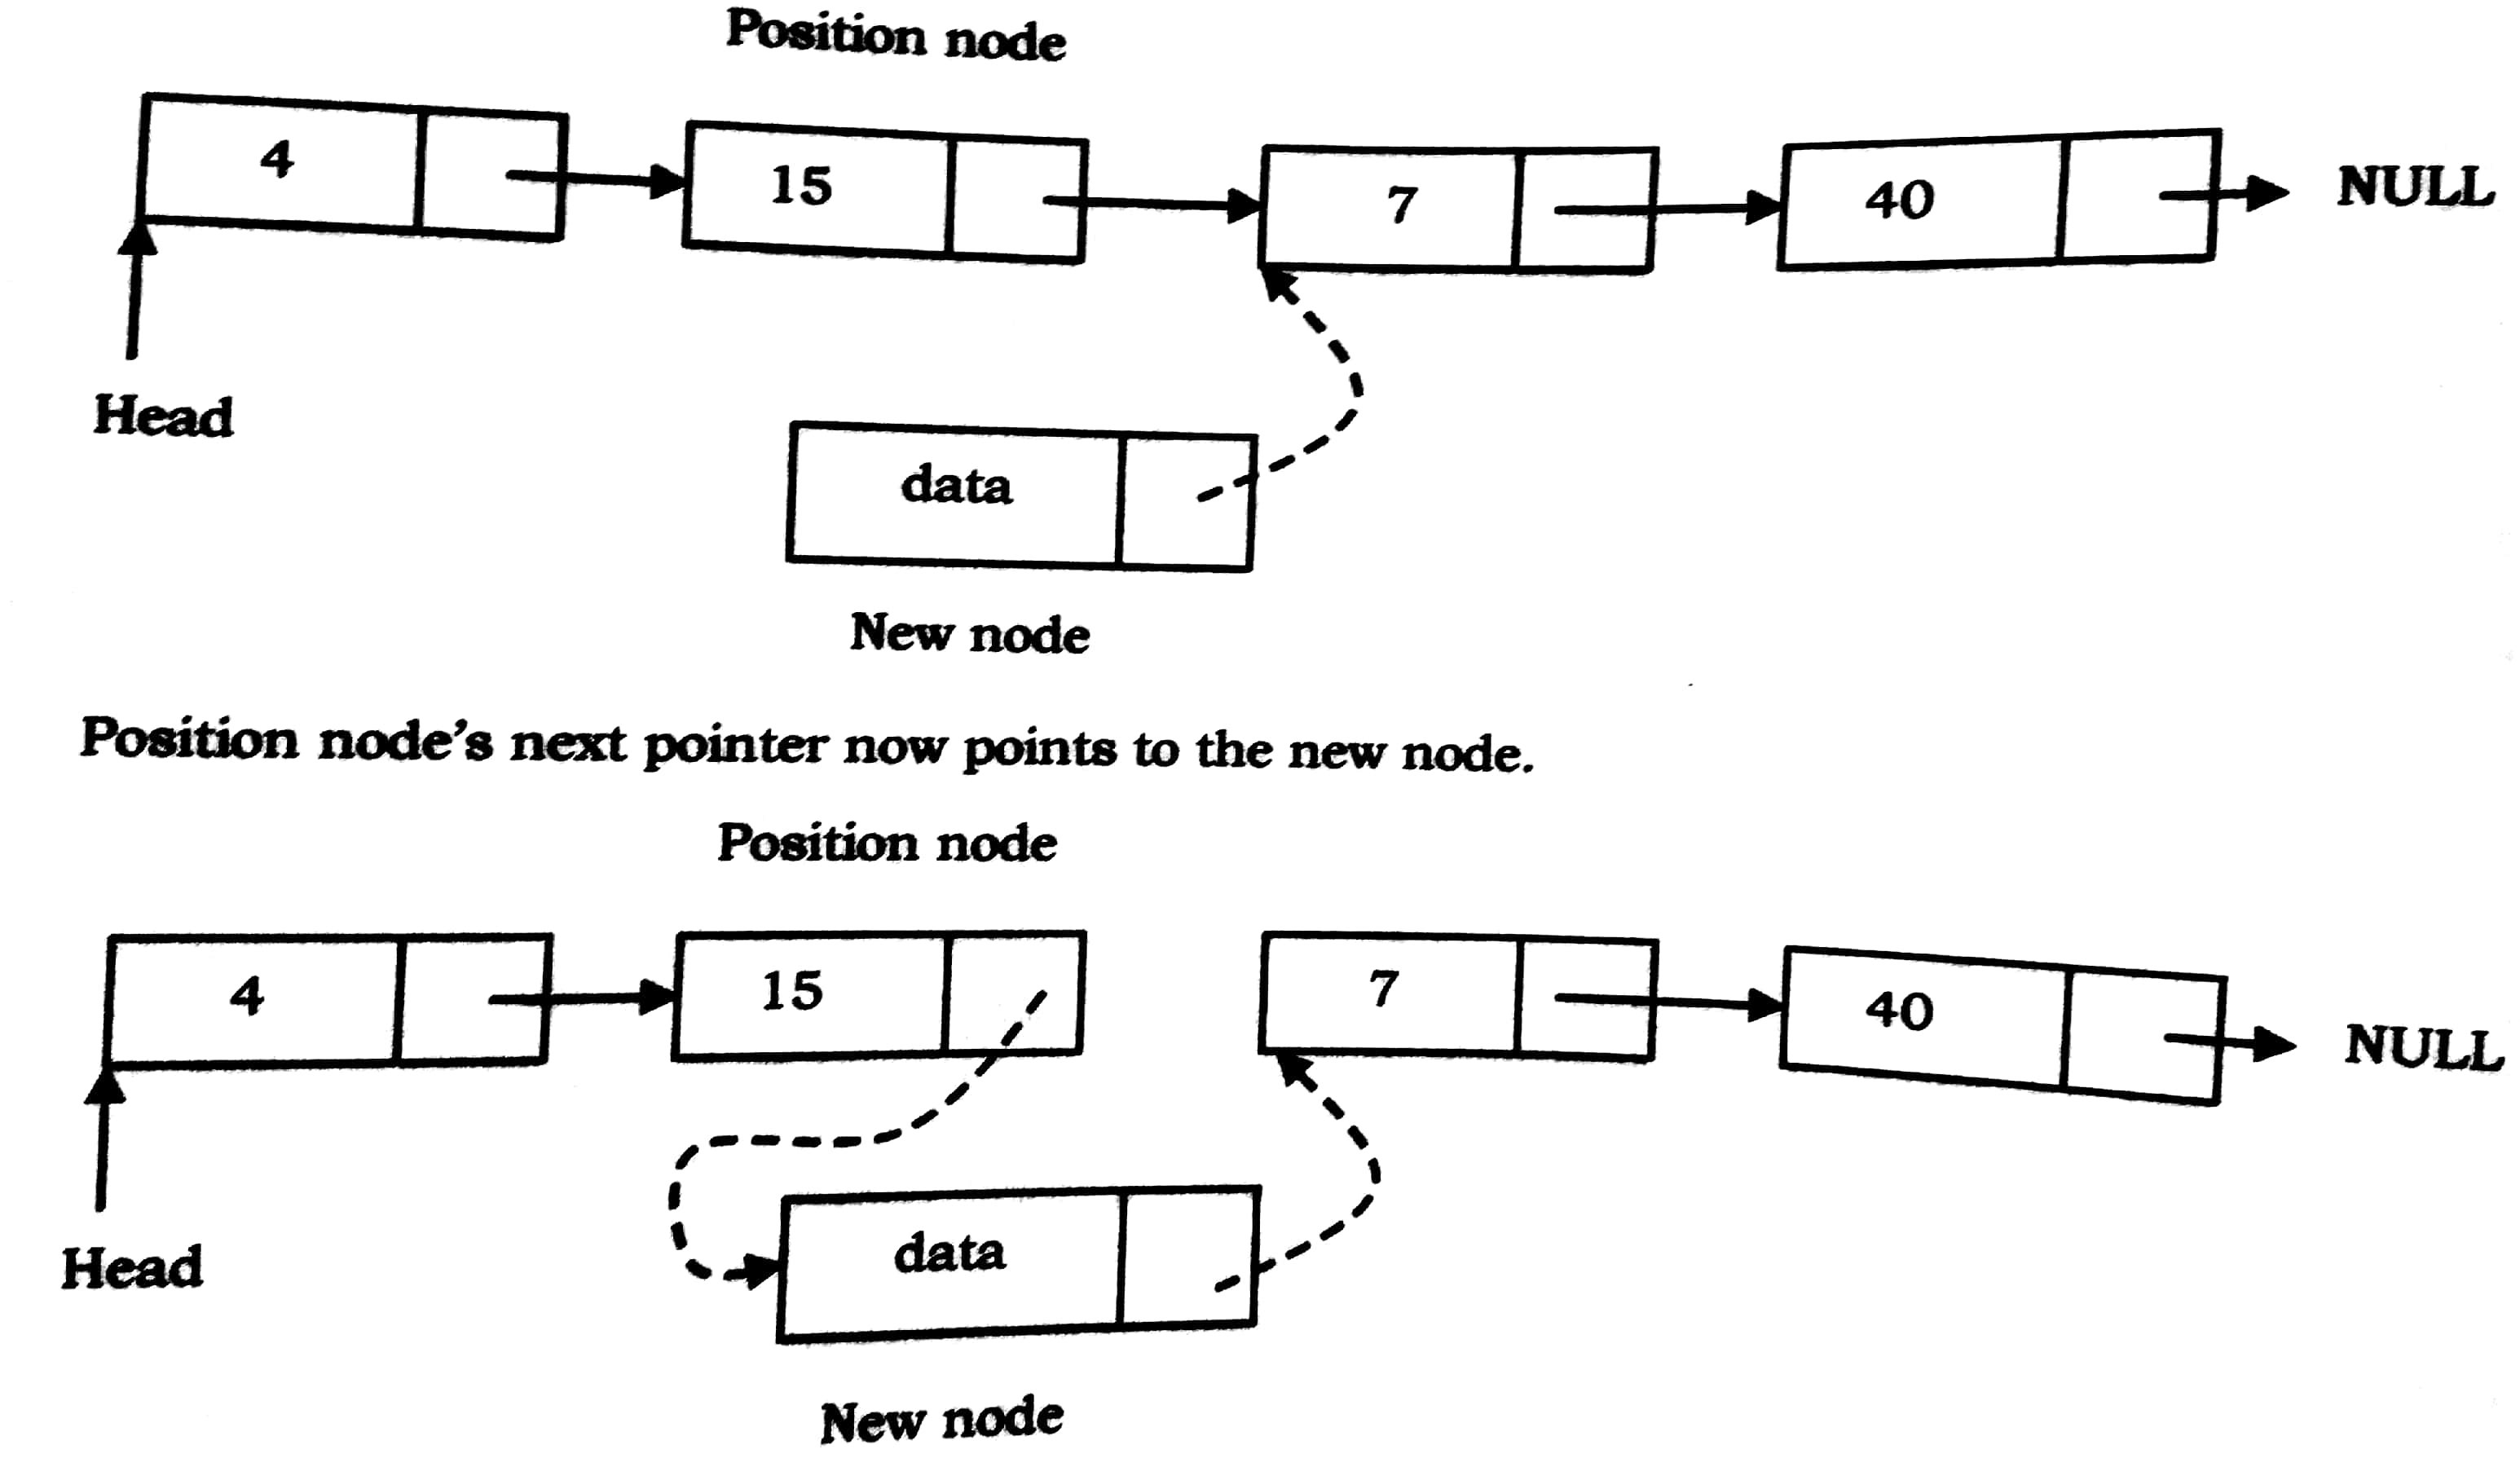
\includegraphics[height=0.50\paperheight, width=0.7\paperwidth]{figs/fig_listas/insere_posicao}						
			\caption{Incluir um nó numa posição da lista}	
%%				\label{fig:lista-linear-repre}
		\end{figure} 

\end{frame} 
%----------------------------------------------------------------------------------------------------------
%[allowframebreaks=0.9]

\begin{frame}%%%[allowframebreaks=0.98]

\frametitle{Excluindo o nó no início da lista -- \textit{cabeça} da lista}

\begin{figure}[!hb]
	\centering
%%		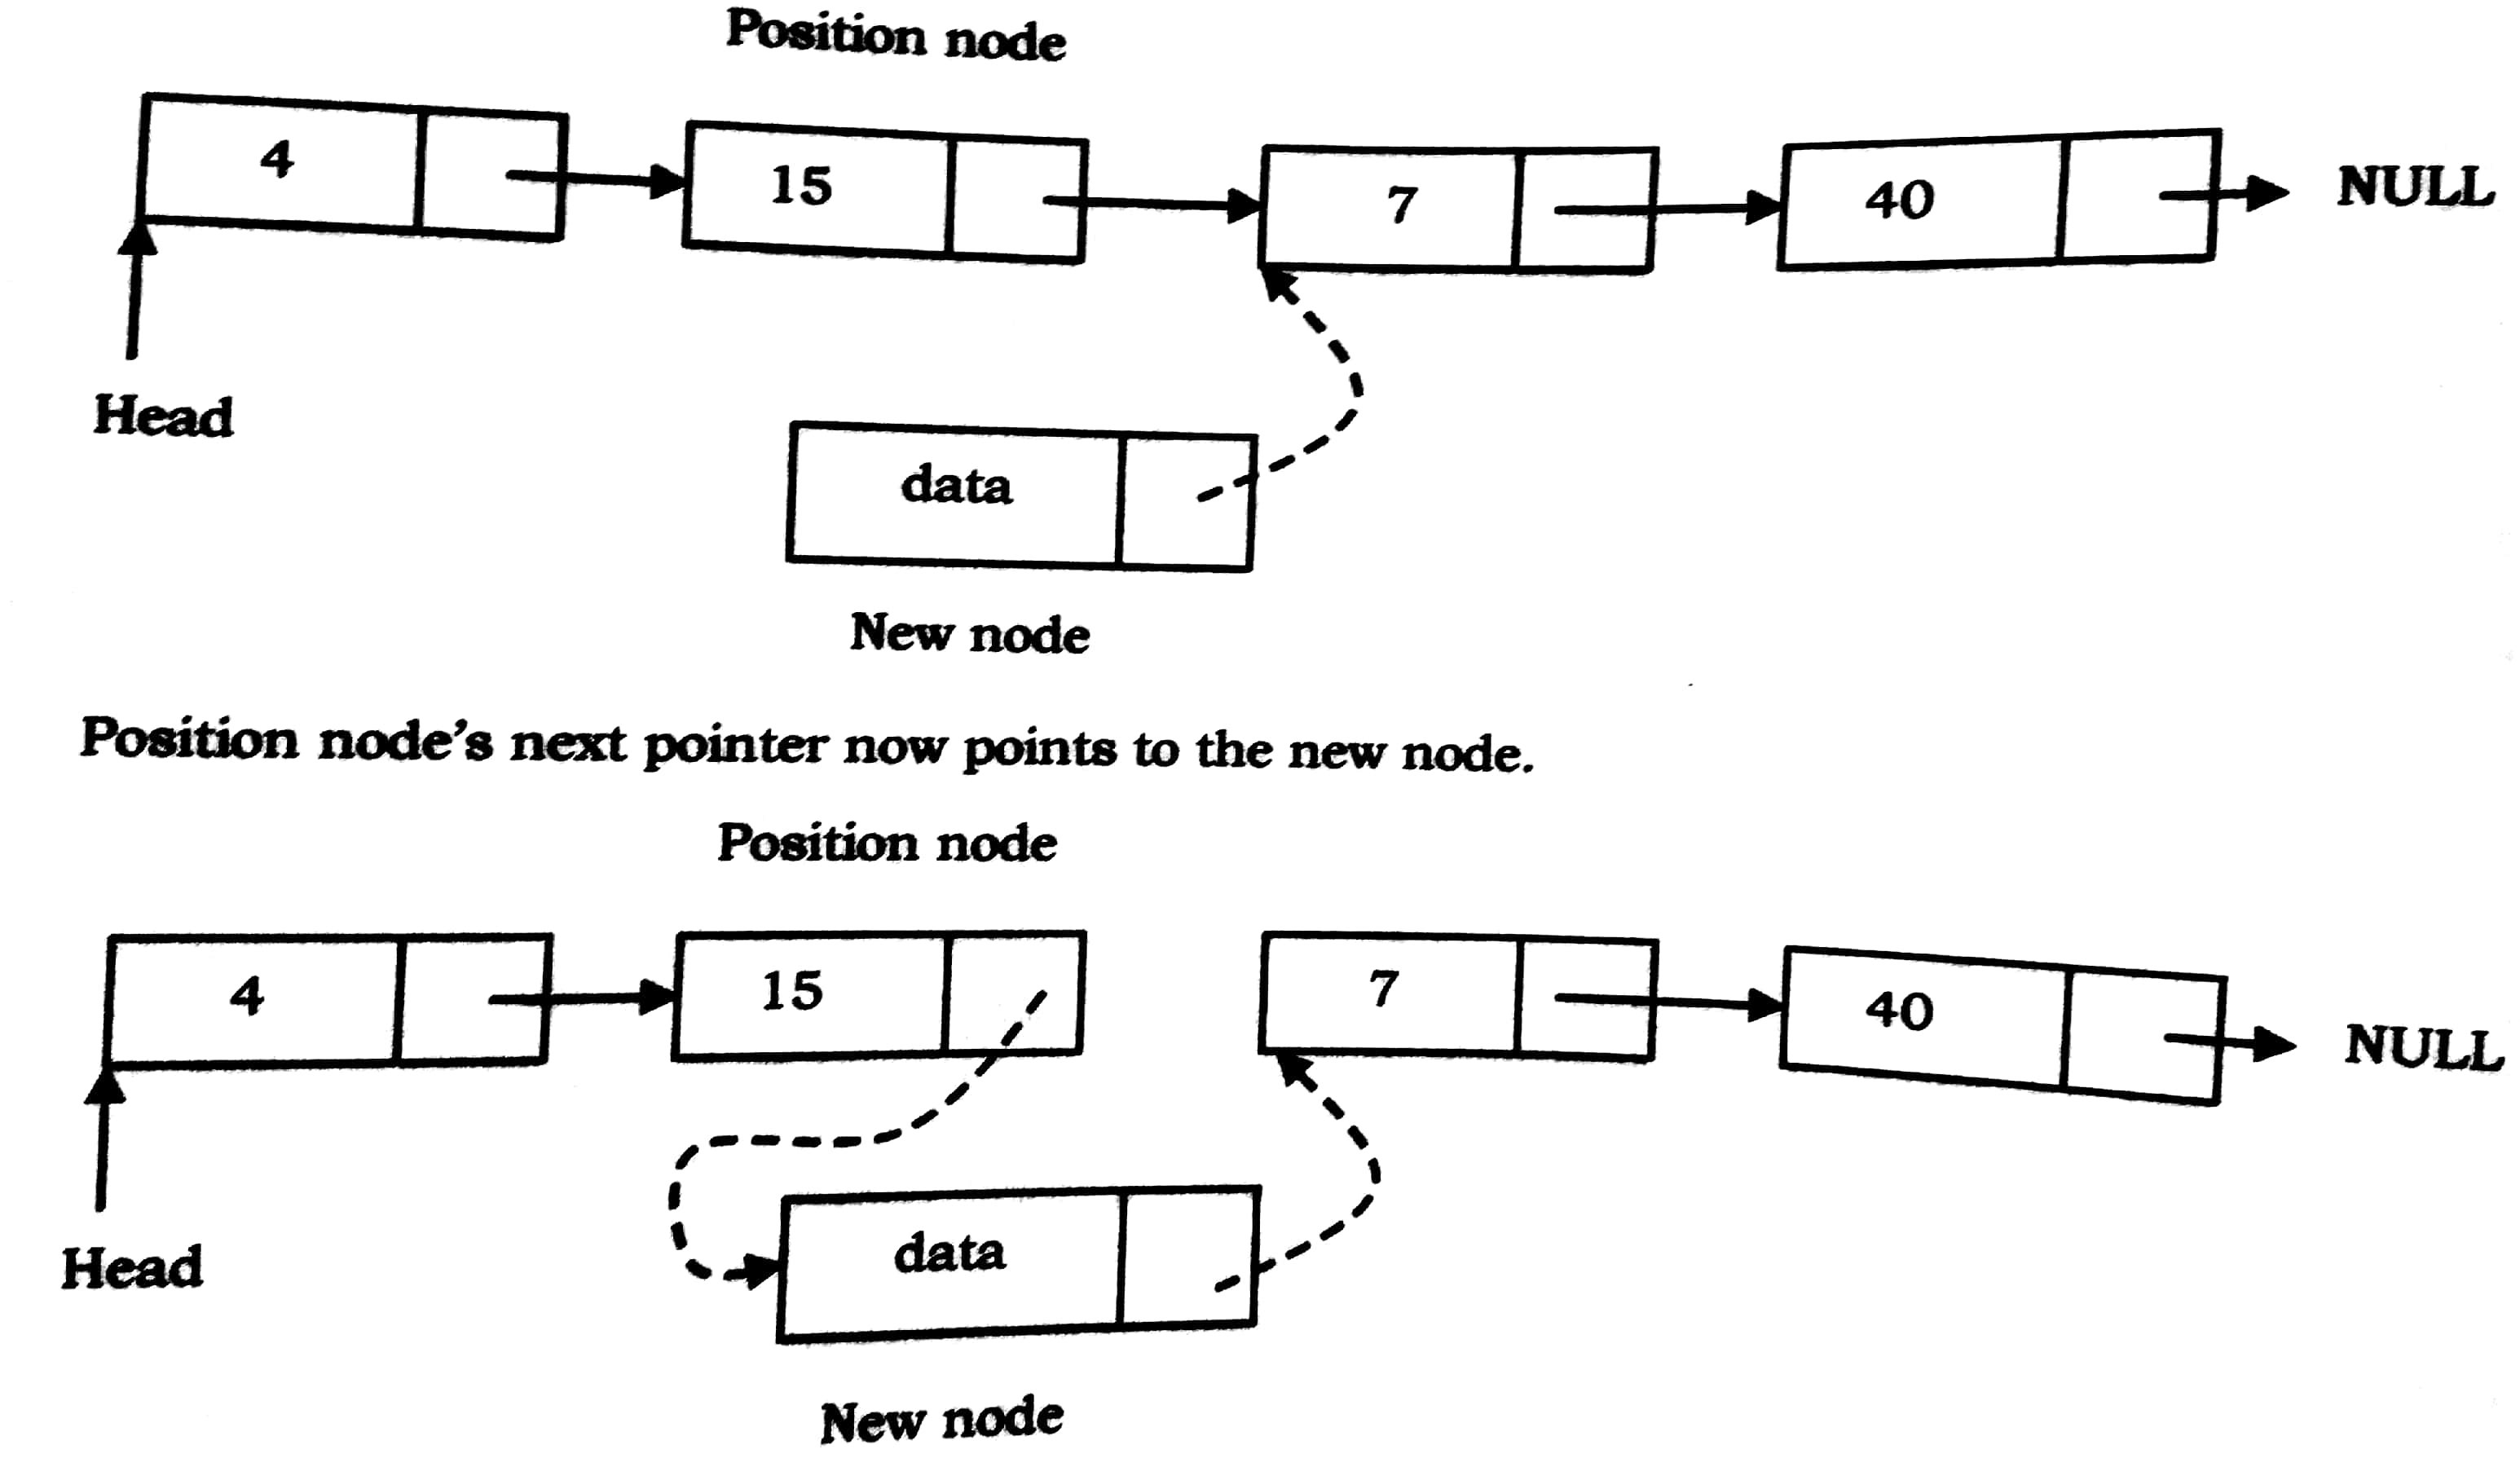
\includegraphics[scale=0.1]{figs/fig_listas/insere_posicao}
	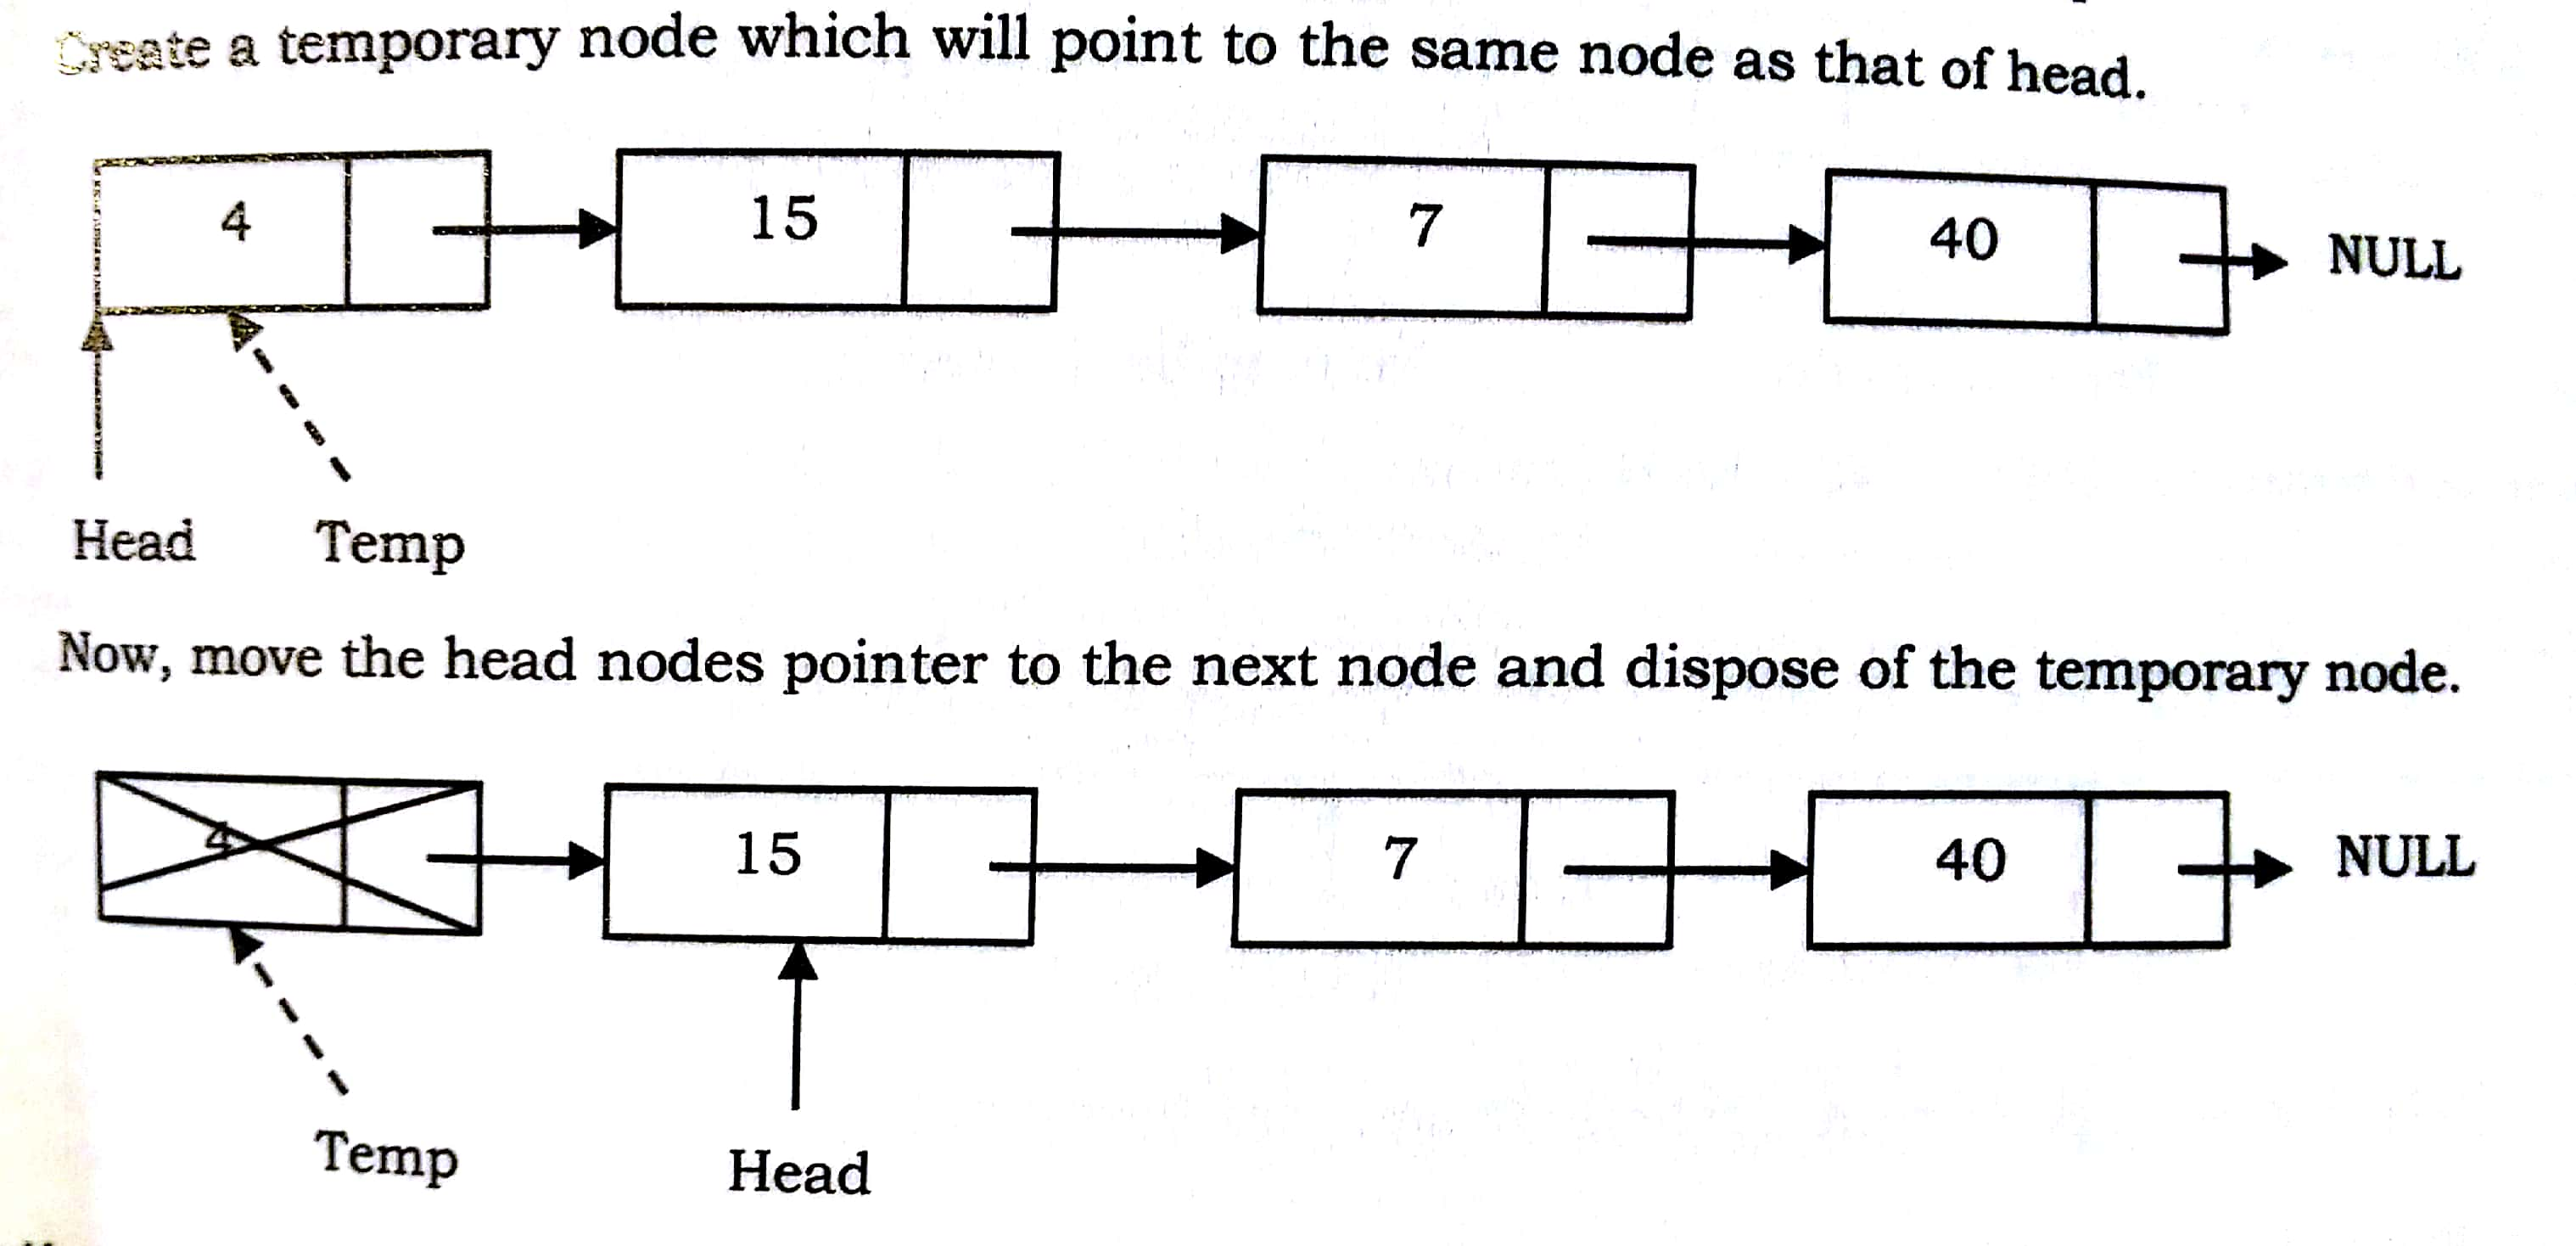
\includegraphics[height=0.50\paperheight, width=0.7\paperwidth]{figs/fig_listas/exclui_inicio}						
			\caption{Exclui o nó no início da lista}	
%%				\label{fig:lista-linear-repre}
		\end{figure} 

\end{frame} 

%----------------------------------------------------------------------------------------------------------

\begin{frame}%%%[allowframebreaks=0.98]

\frametitle{Excluindo um nó no  meio  da lista}

\begin{figure}[!hb]
	\centering
%%		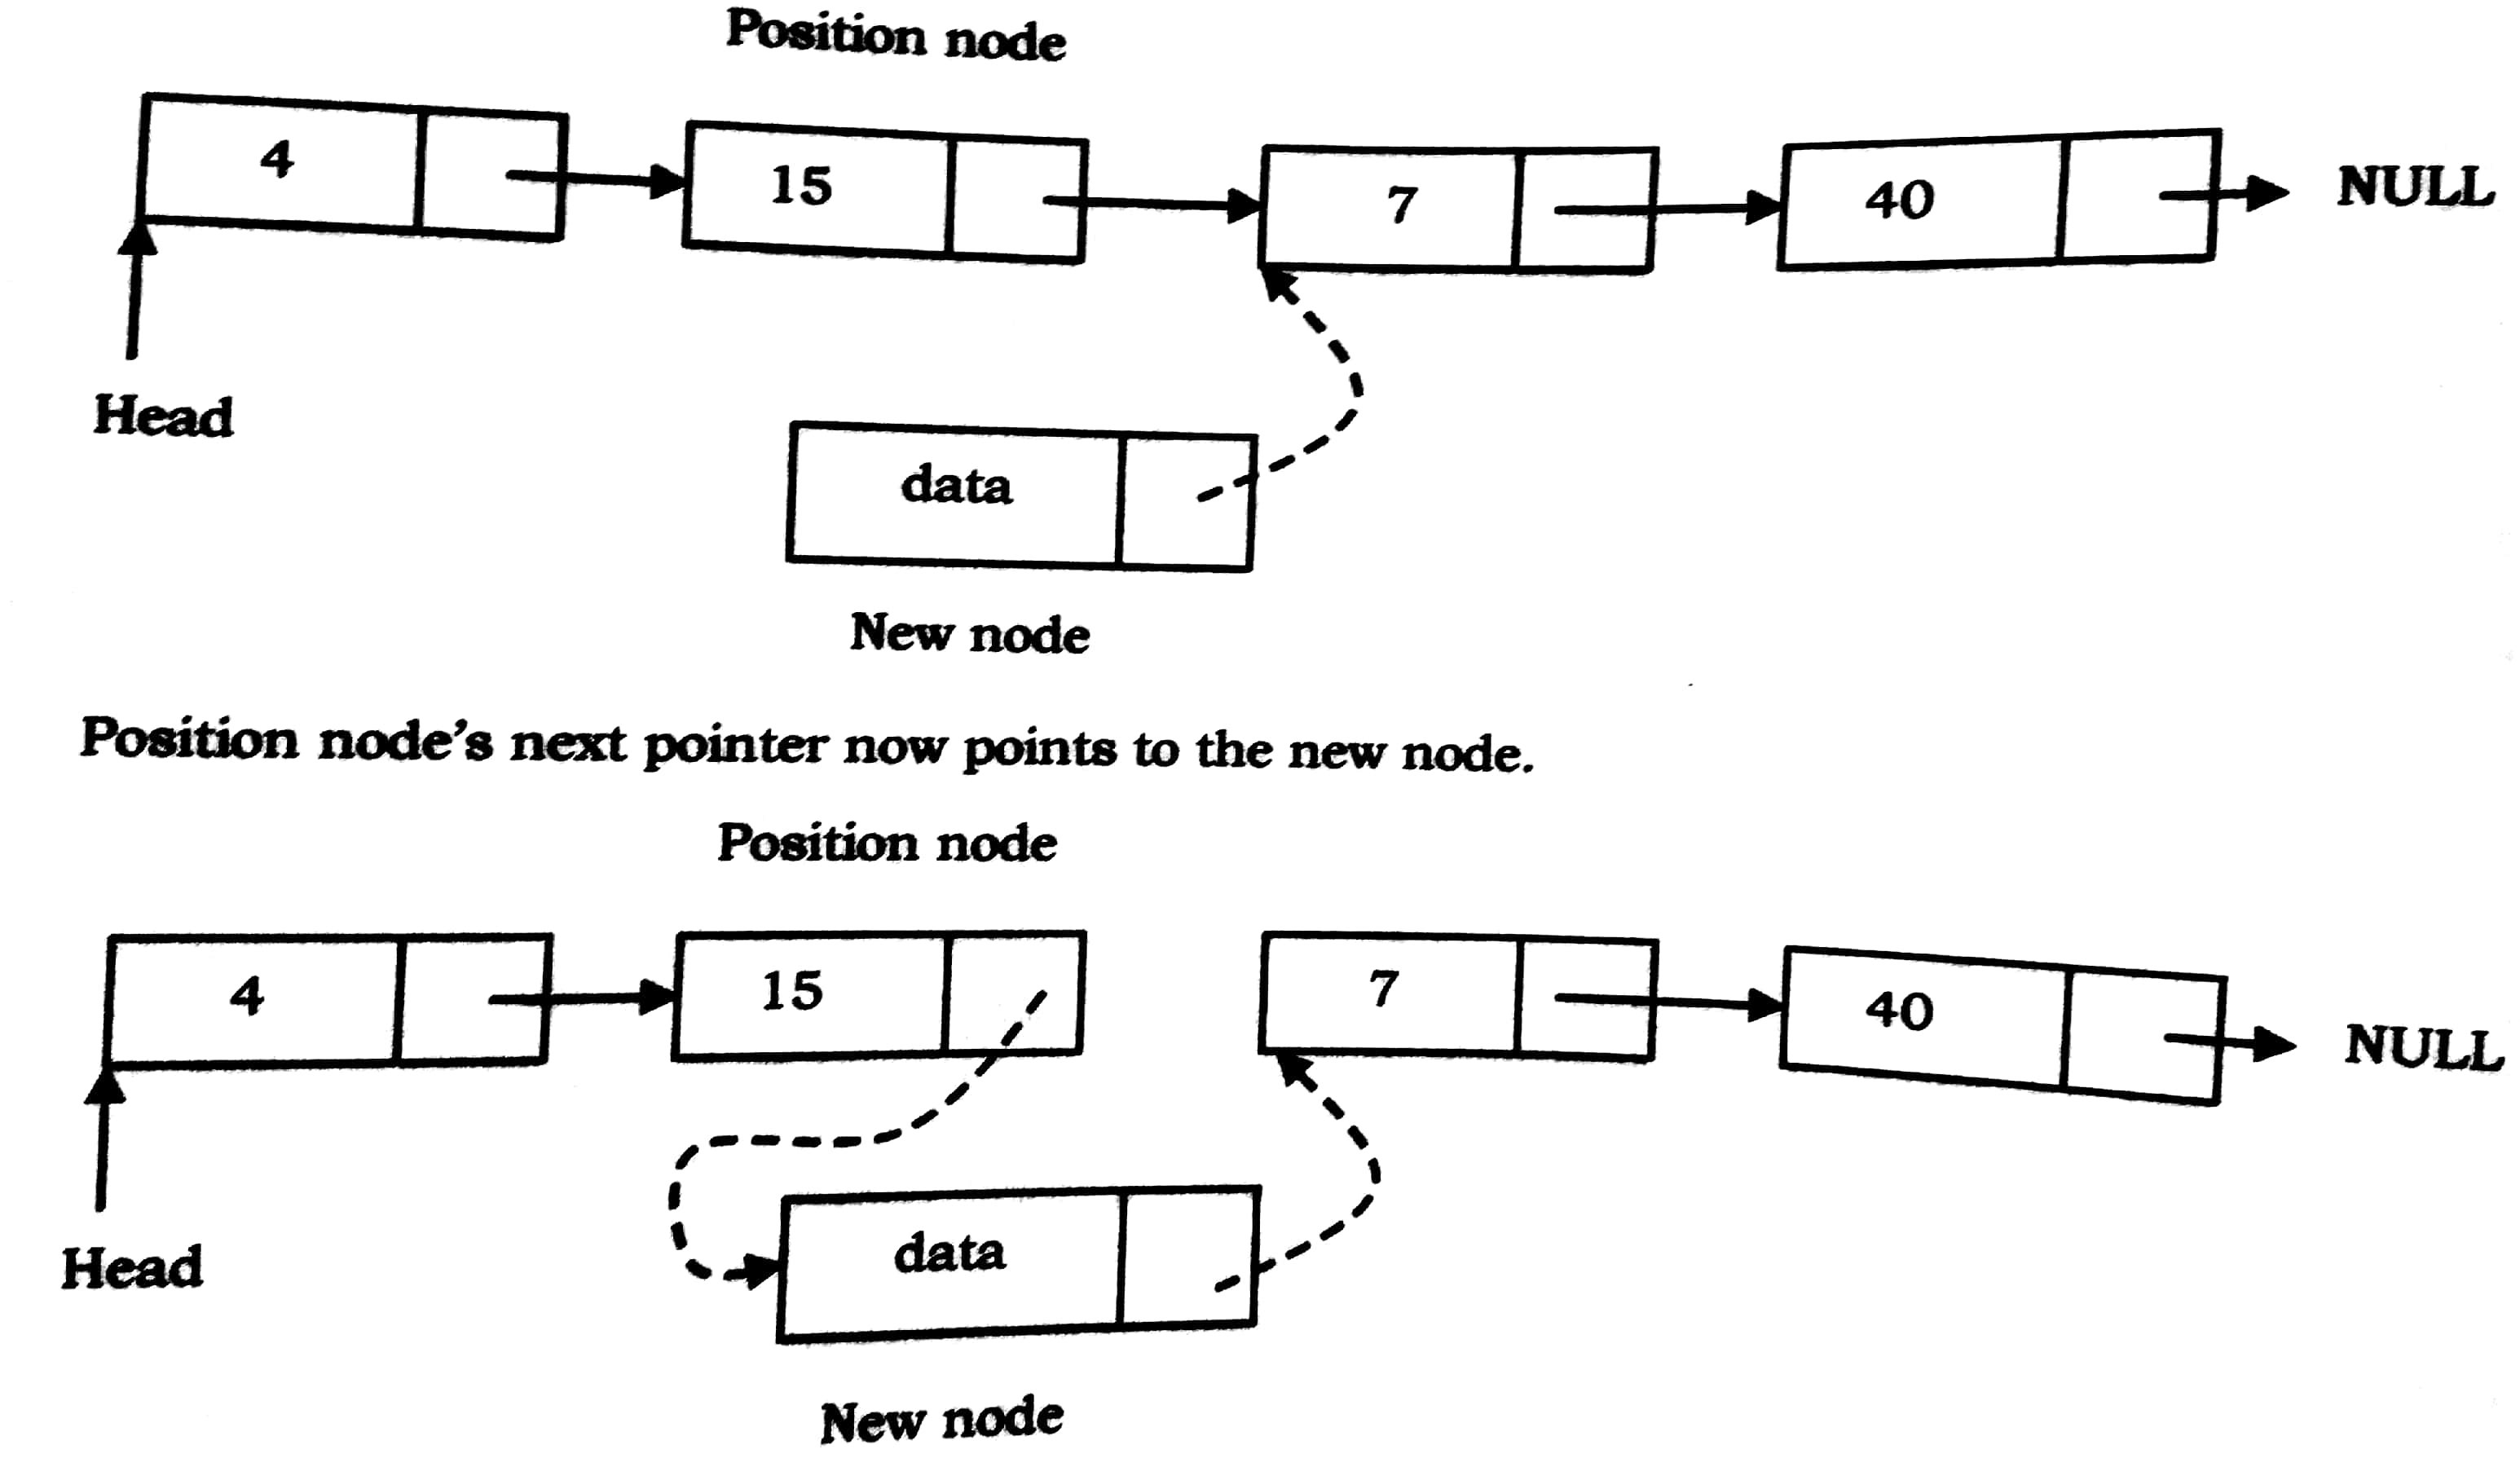
\includegraphics[scale=0.1]{figs/fig_listas/insere_posicao}
	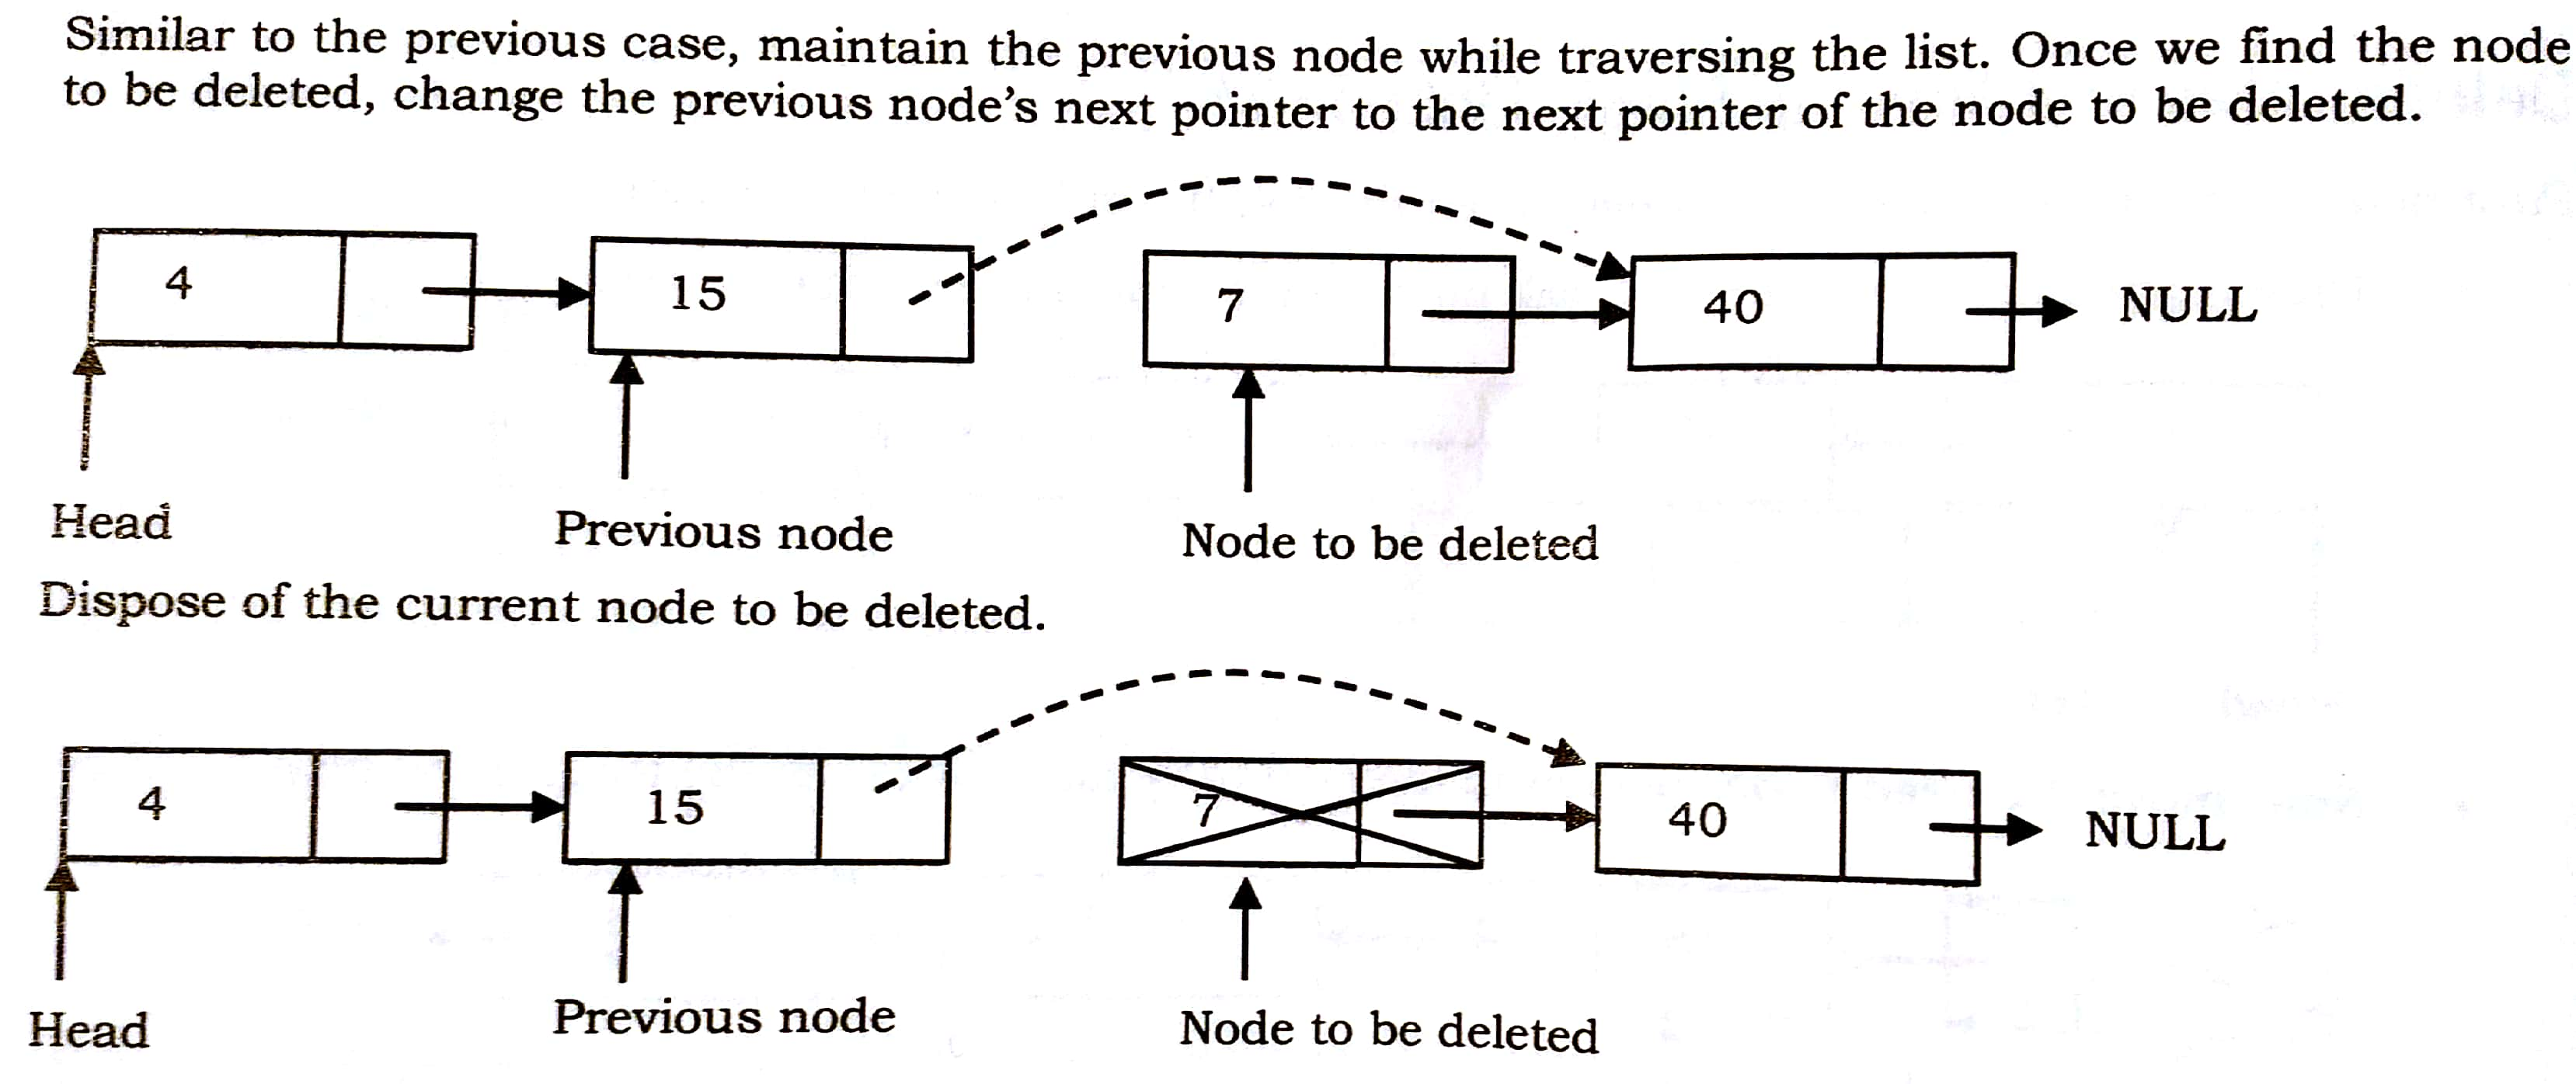
\includegraphics[height=0.50\paperheight, width=0.7\paperwidth]{figs/fig_listas/exclui_no_meio}						
			\caption{Exclui nó no  meio  da lista -- k-ésima posição ou por conteúdo}	
%%				\label{fig:lista-linear-repre}
		\end{figure} 

\end{frame} 

%----------------------------------------------------------------------------------------------------------

\begin{frame}%%%[allowframebreaks=0.98]

\frametitle{Excluindo o último nó da lista}

\begin{figure}[!hb]
	\centering
%%		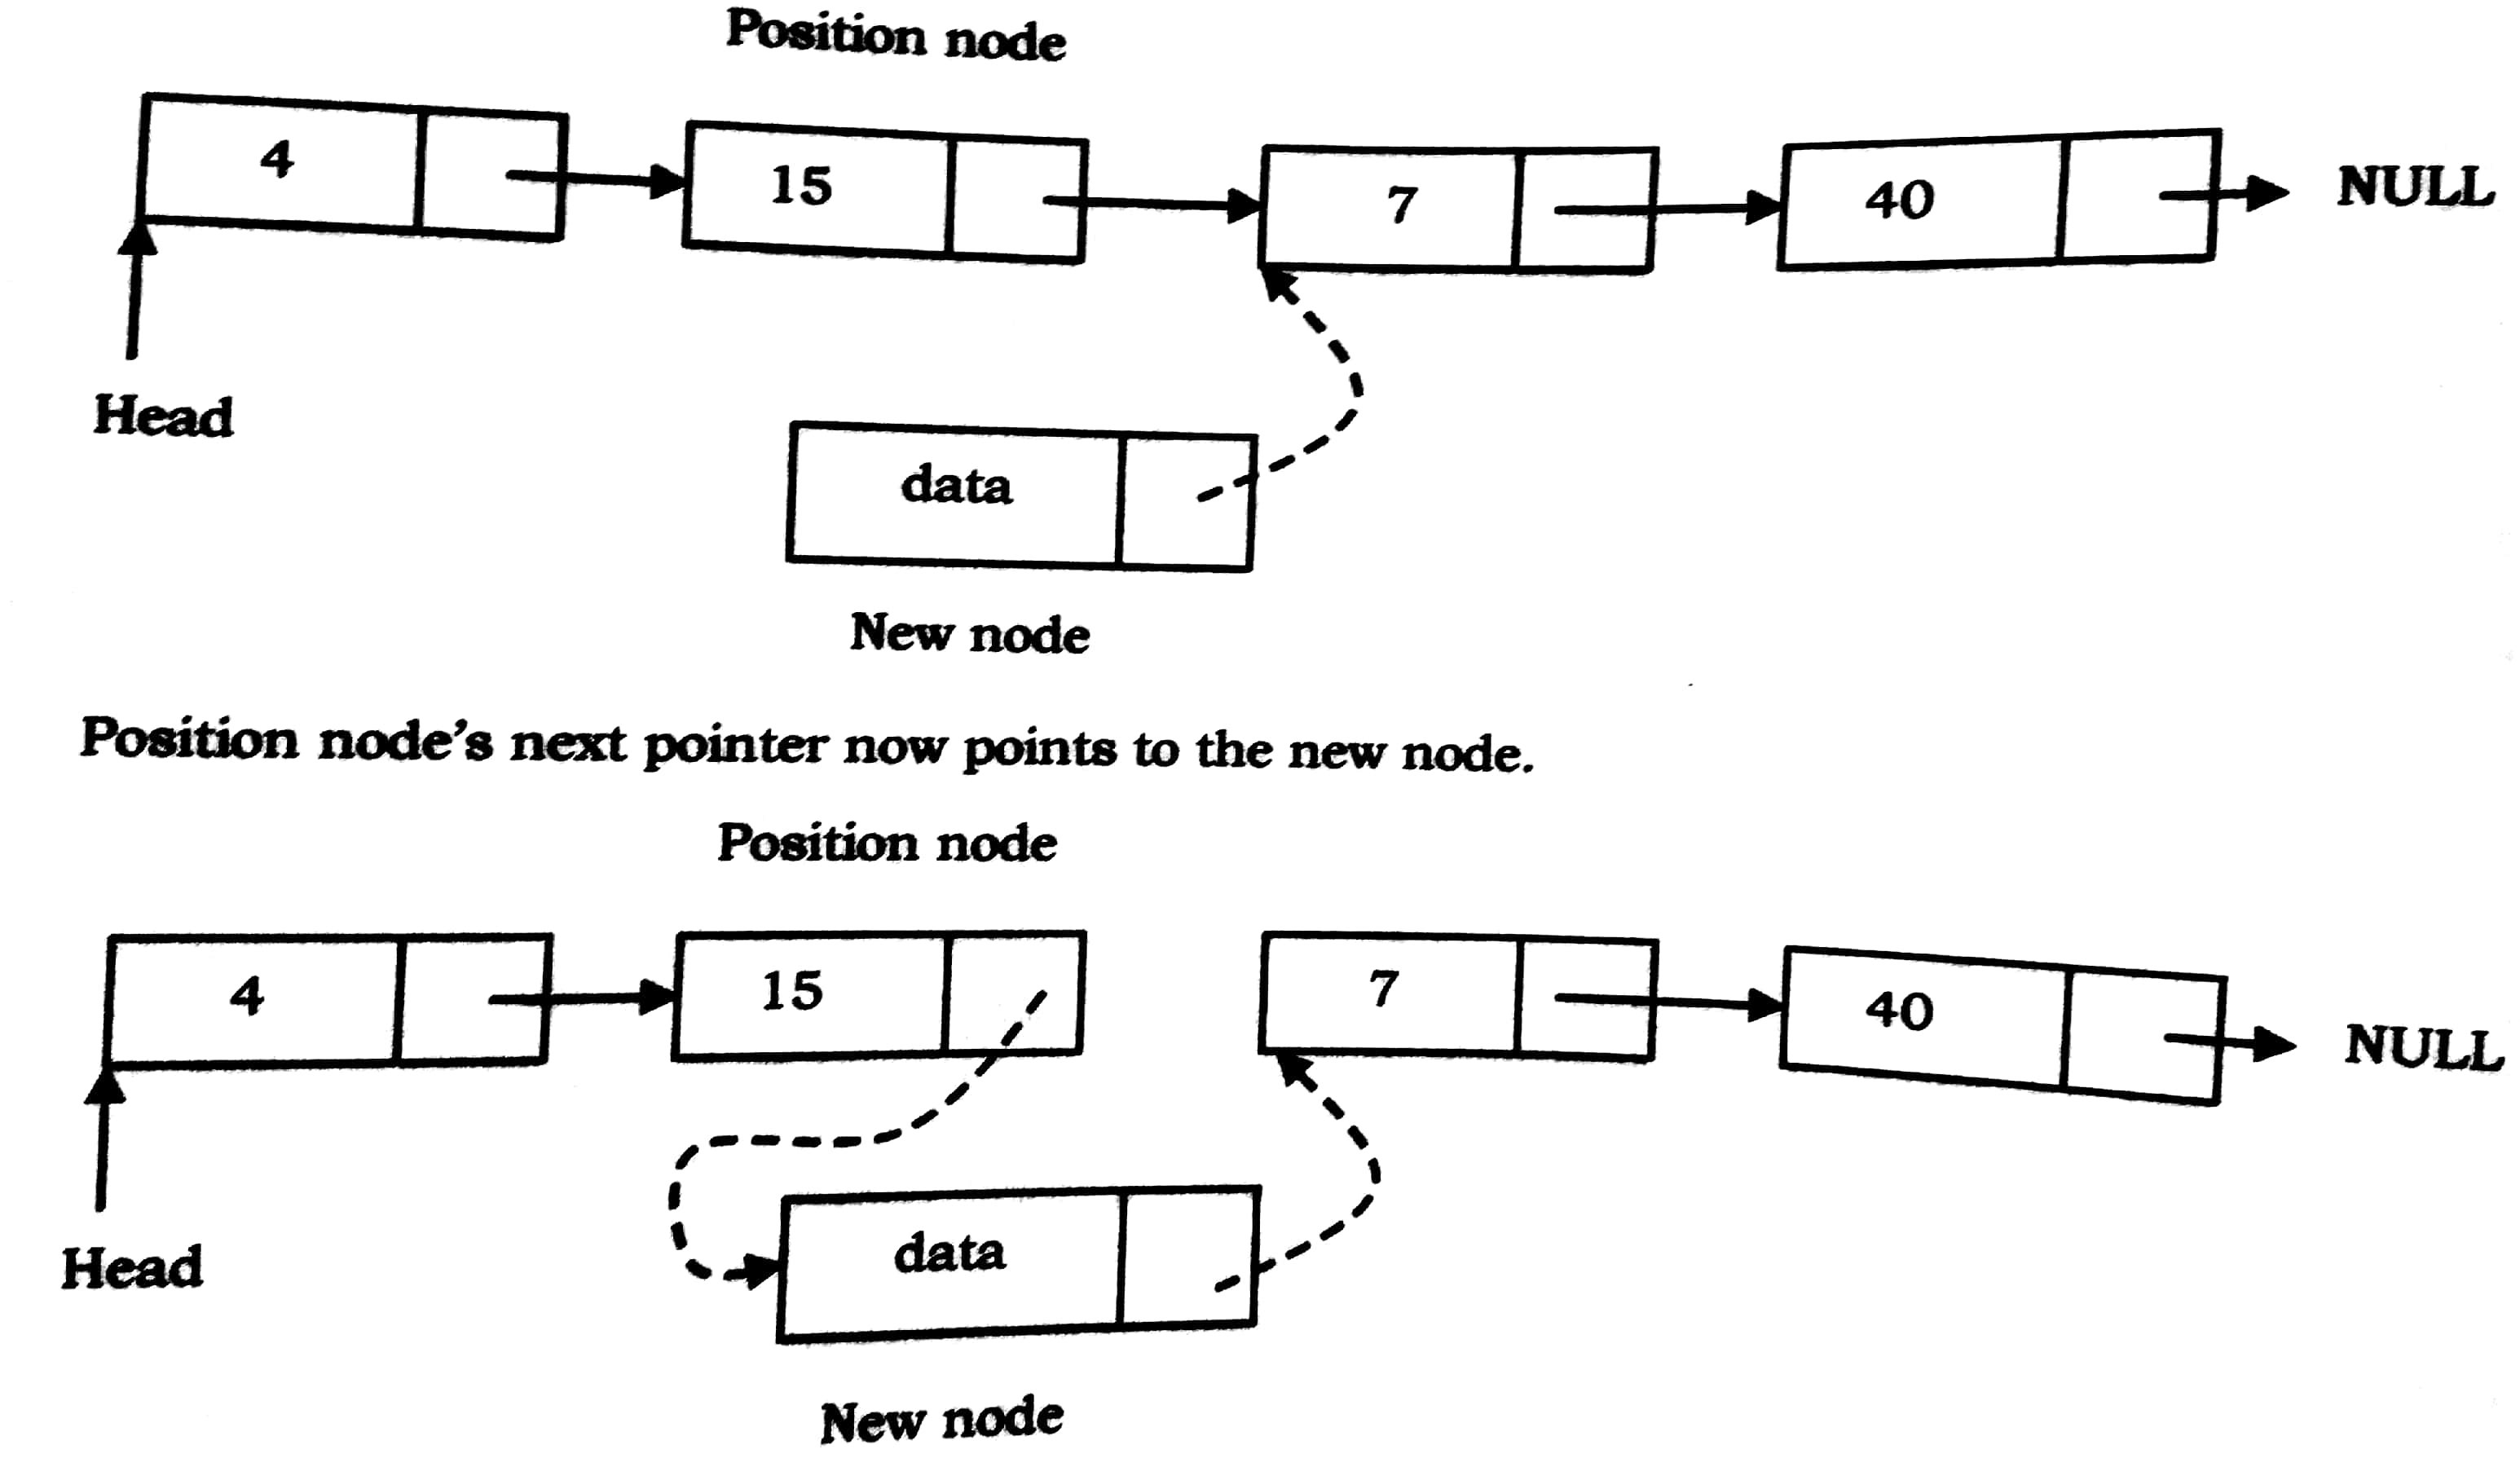
\includegraphics[scale=0.1]{figs/fig_listas/insere_posicao}
	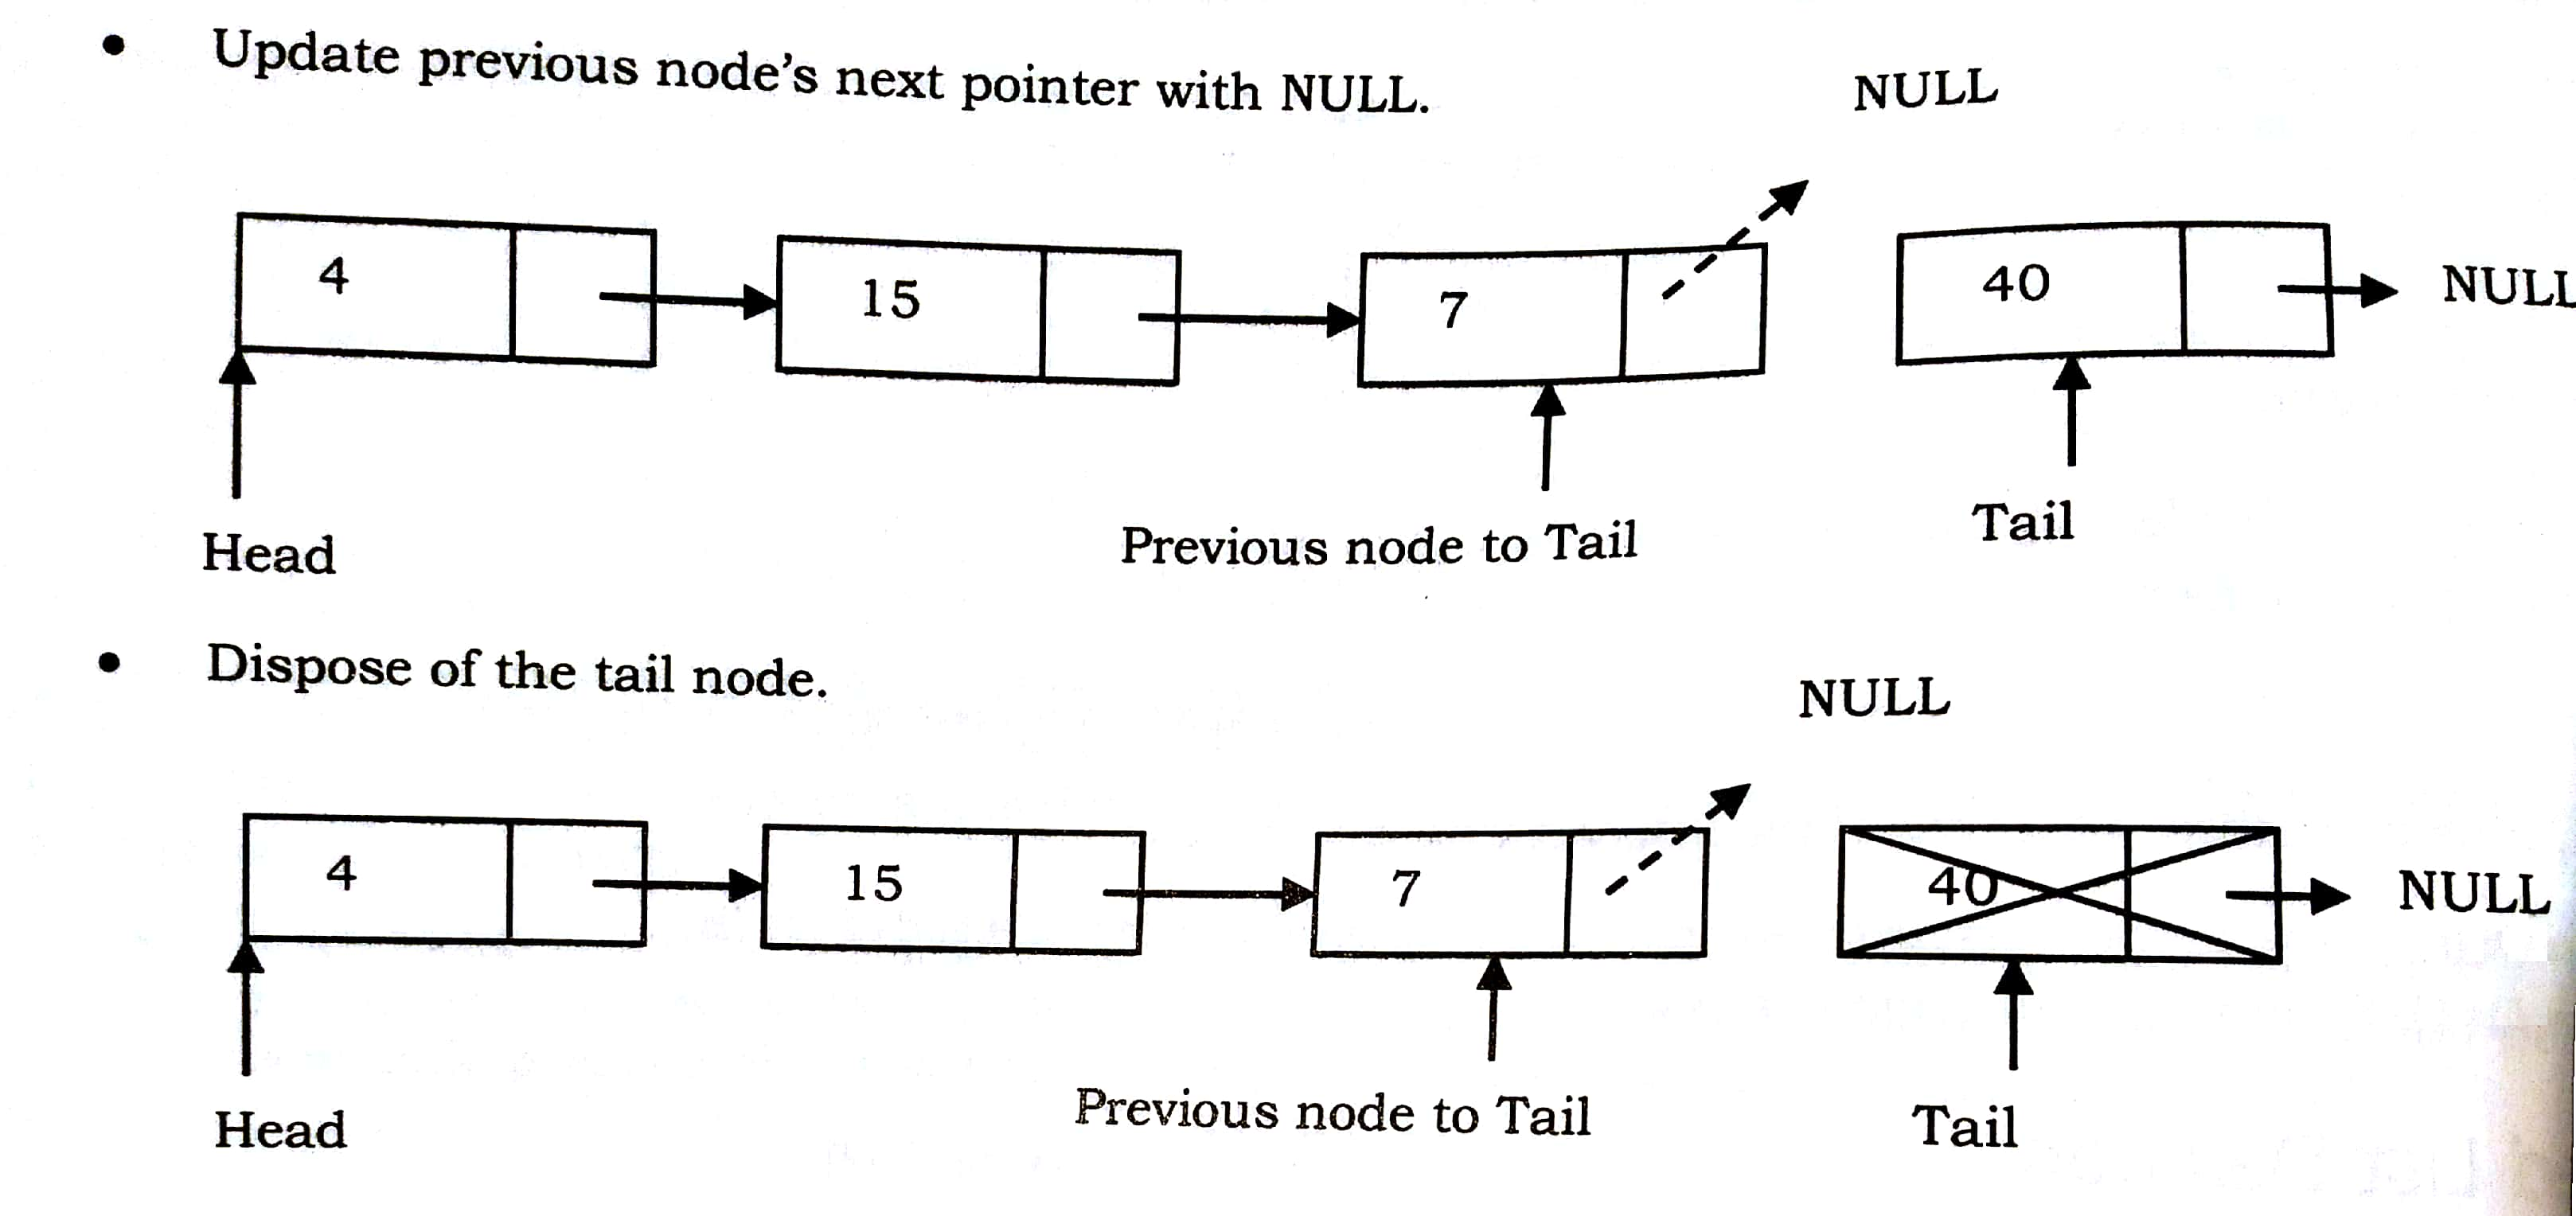
\includegraphics[height=0.50\paperheight, width=0.7\paperwidth]{figs/fig_listas/exclui_ultimo_no}						
			\caption{Exclui o último nó da lista}	
%%				\label{fig:lista-linear-repre}
		\end{figure} 

\end{frame} 



%----------------------------------------------------------------------------------------------------------

\begin{frame}%%%[allowframebreaks=0.98]

\frametitle{Listas Duplamente Encadeadas -- LDE}

\begin{figure}[!hb]
	\centering
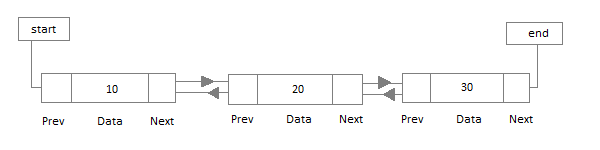
\includegraphics[height=0.450\paperheight, width=0.8\paperwidth]{figs/fig_listas/lista_DE_01.png}						
			\caption{Listas Duplamente Encadeadas -- LDE}	
%%				\label{fig:lista-linear-repre}
		\end{figure} 

\begin{itemize}
  \item Para onde estão apontando  o primeiro e o último  ponteiro ?
  \item Podem ser circulares?
\end{itemize}
\end{frame} 


%----------------------------------------------------------------------------------------------------------


\begin{frame}%%%[allowframebreaks=0.98]

\frametitle{Inserindo um nó em listas duplamente encadeadas -- LDE}

\begin{figure}[!hb]
	\centering

	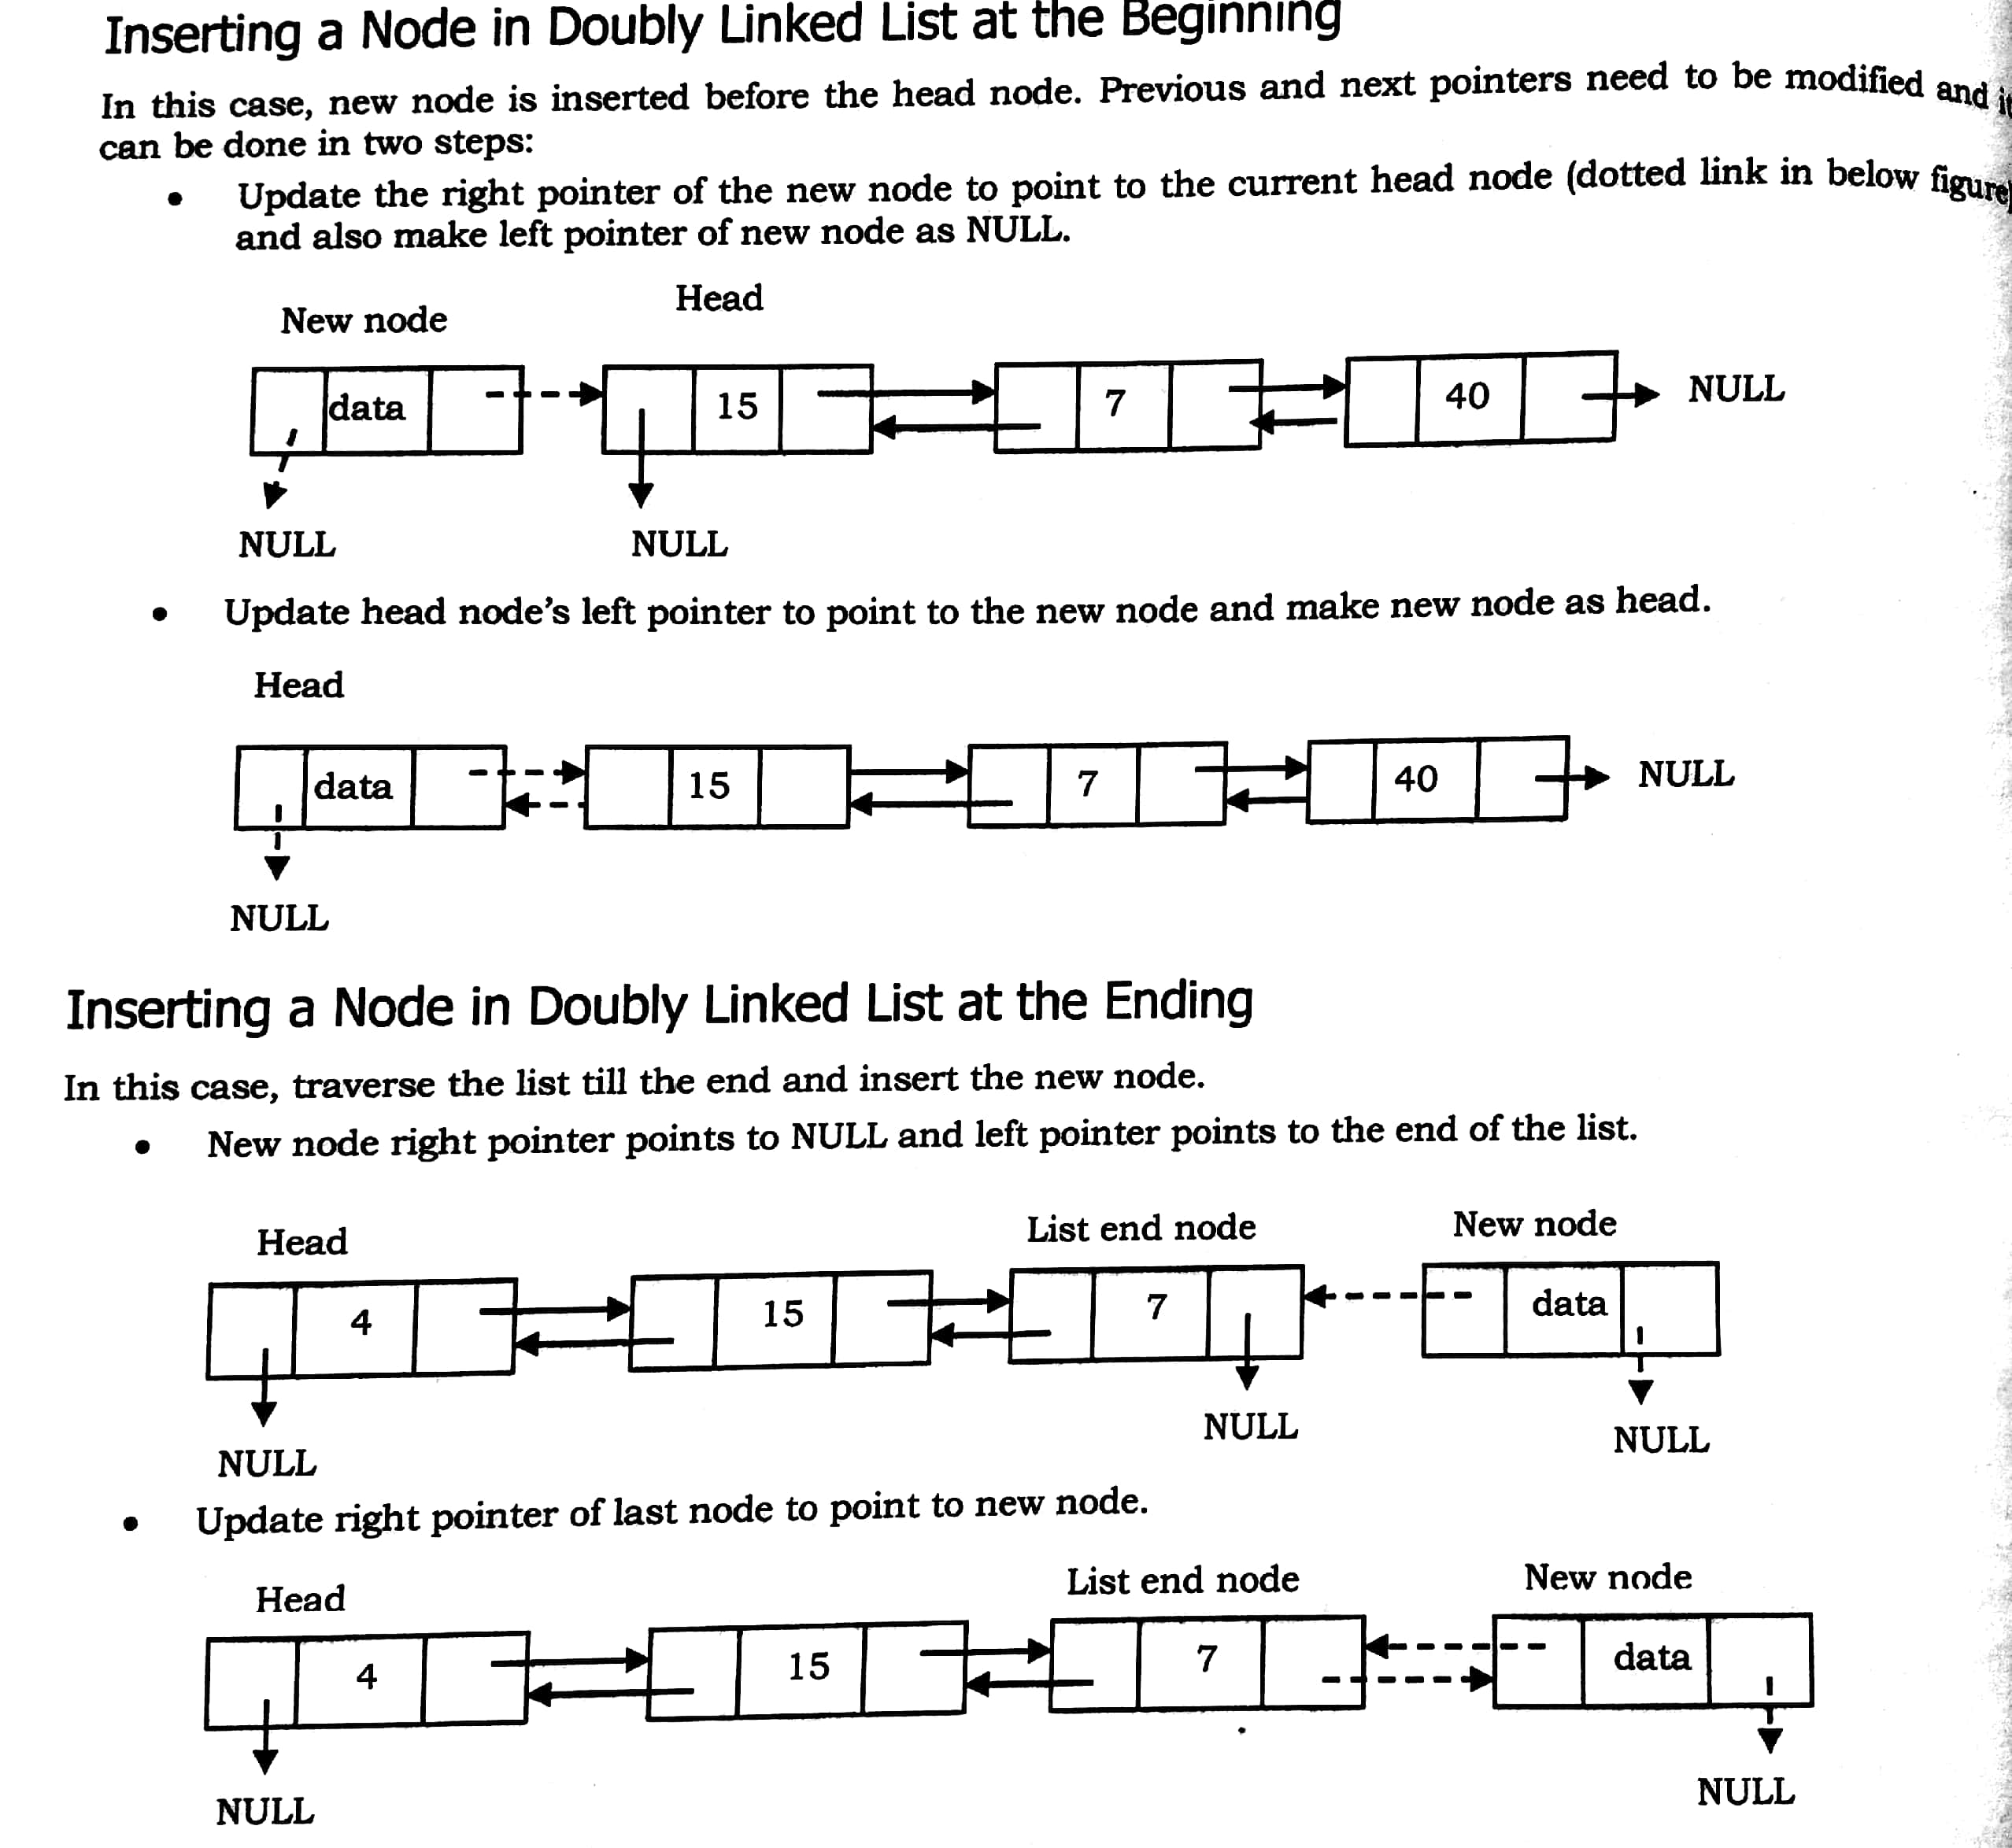
\includegraphics[height=0.650\paperheight, width=0.77\paperwidth]{figs/fig_listas/insercao_LDE}						
			\caption{Incluindo um nó numa LDE}	
%%				\label{fig:lista-linear-repre}
		\end{figure} 

\end{frame} 
%----------------------------------------------------------------------------------------------------------
%[allowframebreaks=0.9]


%----------------------------------------------------------------------------------------------------------

\begin{frame}%%%[allowframebreaks=0.98]

\frametitle{Listas Circulares}

\begin{figure}[!hb]
	\centering
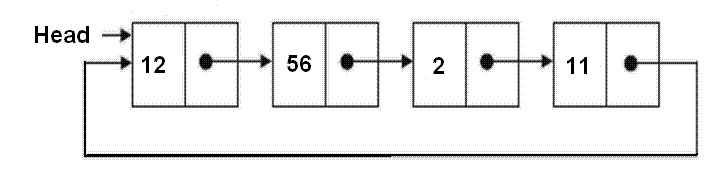
\includegraphics[height=0.30\paperheight, width=0.9\paperwidth]{figs/fig_listas/lista_circular.jpg}						
			\caption{Listas Circulares}	
%%				\label{fig:lista-linear-repre}
		\end{figure} 

\end{frame} 

\begin{frame}%%%[allowframebreaks=0.98]

\frametitle{Excluindo o nó \textit{cabeça} de lista}

\begin{figure}[!hb]
	\centering
	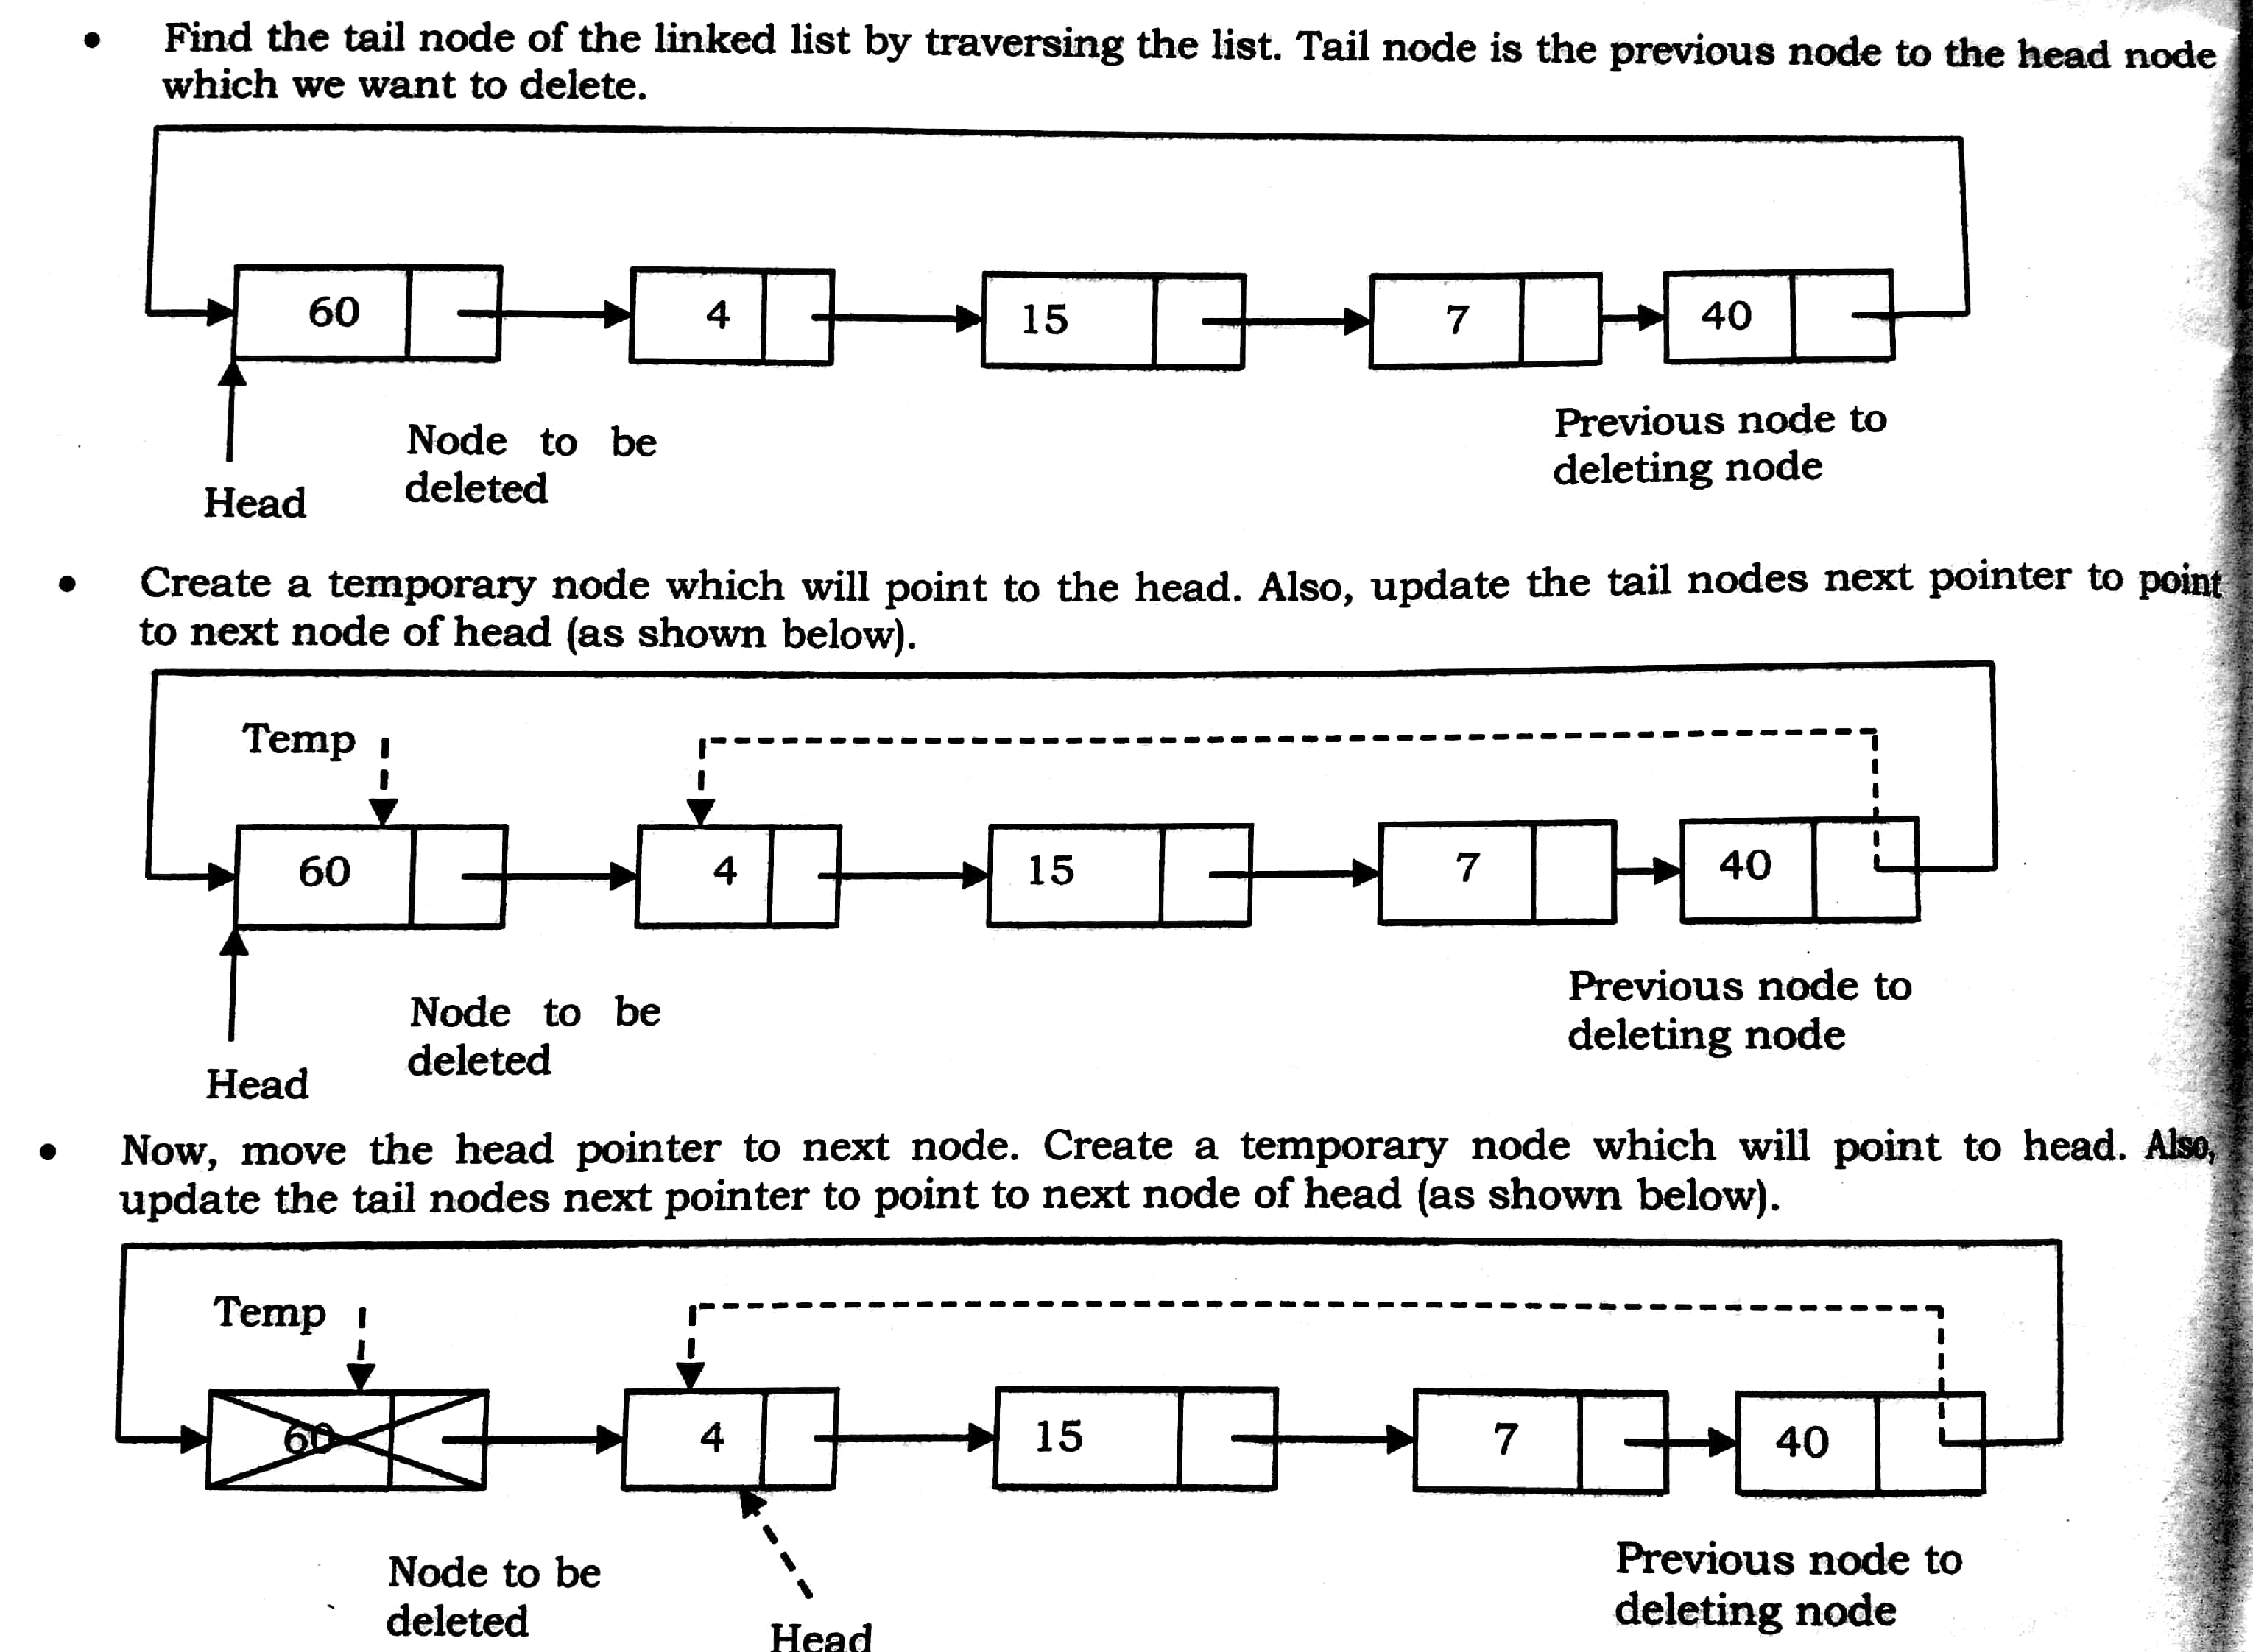
\includegraphics[height=0.650\paperheight, width=0.67\paperwidth]{figs/fig_listas/exclui_1o_no_lista_circular}						
			\caption{Exclui o nó do início da lista}	
%%				\label{fig:lista-linear-repre}
		\end{figure} 

\end{frame} 

%----------------------------------------------------------------------------------------------------------

\begin{frame}%%%[allowframebreaks=0.98]

\frametitle{Listas Mistas}

\begin{figure}[!hb]
	\centering
%%		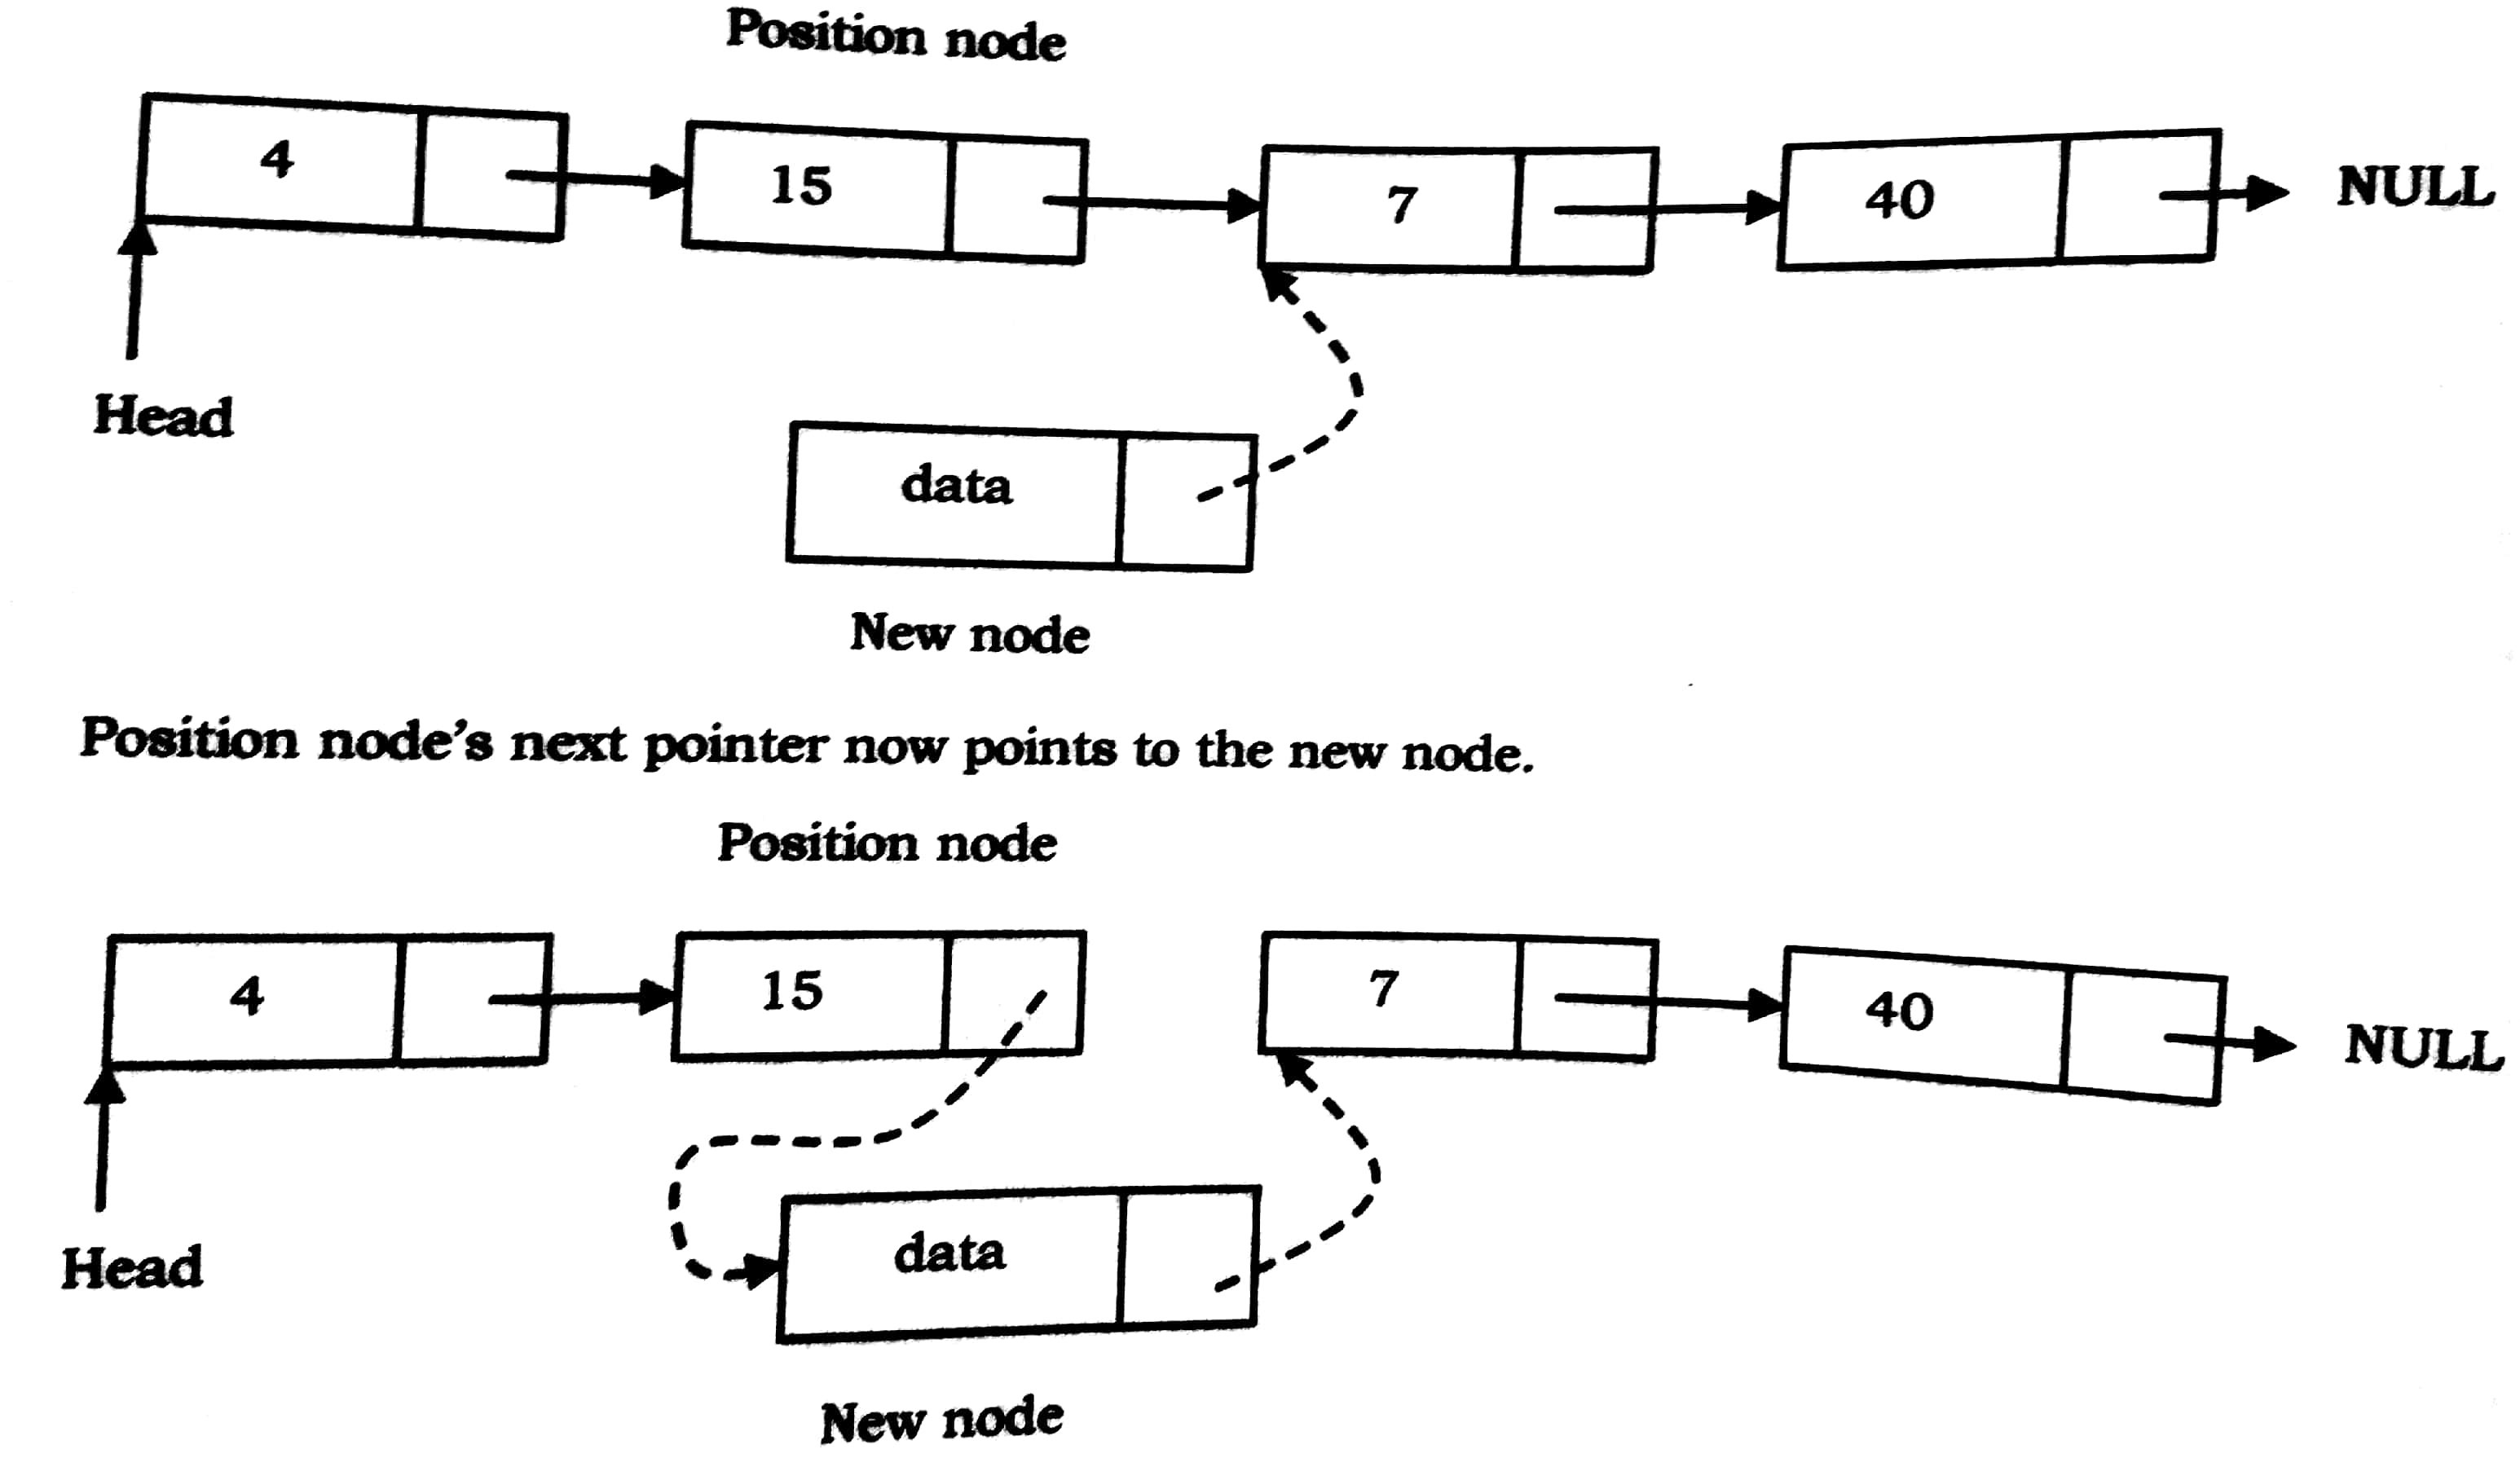
\includegraphics[scale=0.1]{figs/fig_listas/insere_posicao}
	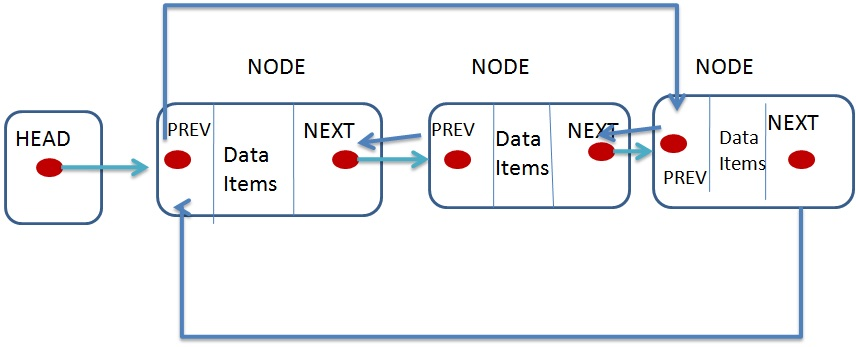
\includegraphics[height=0.450\paperheight, width=0.8\paperwidth]{figs/fig_listas/lista_circular_DE.jpg}						
			\caption{Listas Mistas -- DE e Circular}	
%%				\label{fig:lista-linear-repre}
		\end{figure} 

\end{frame} 

%----------------------------------------------------------------------------------------------------------
\begin{frame}%%%[allowframebreaks=0.98]

\frametitle{Listas Blocadas ou Encapsuladas -- \textit{enrolled}}

\begin{figure}[!hb]
	\centering
%%		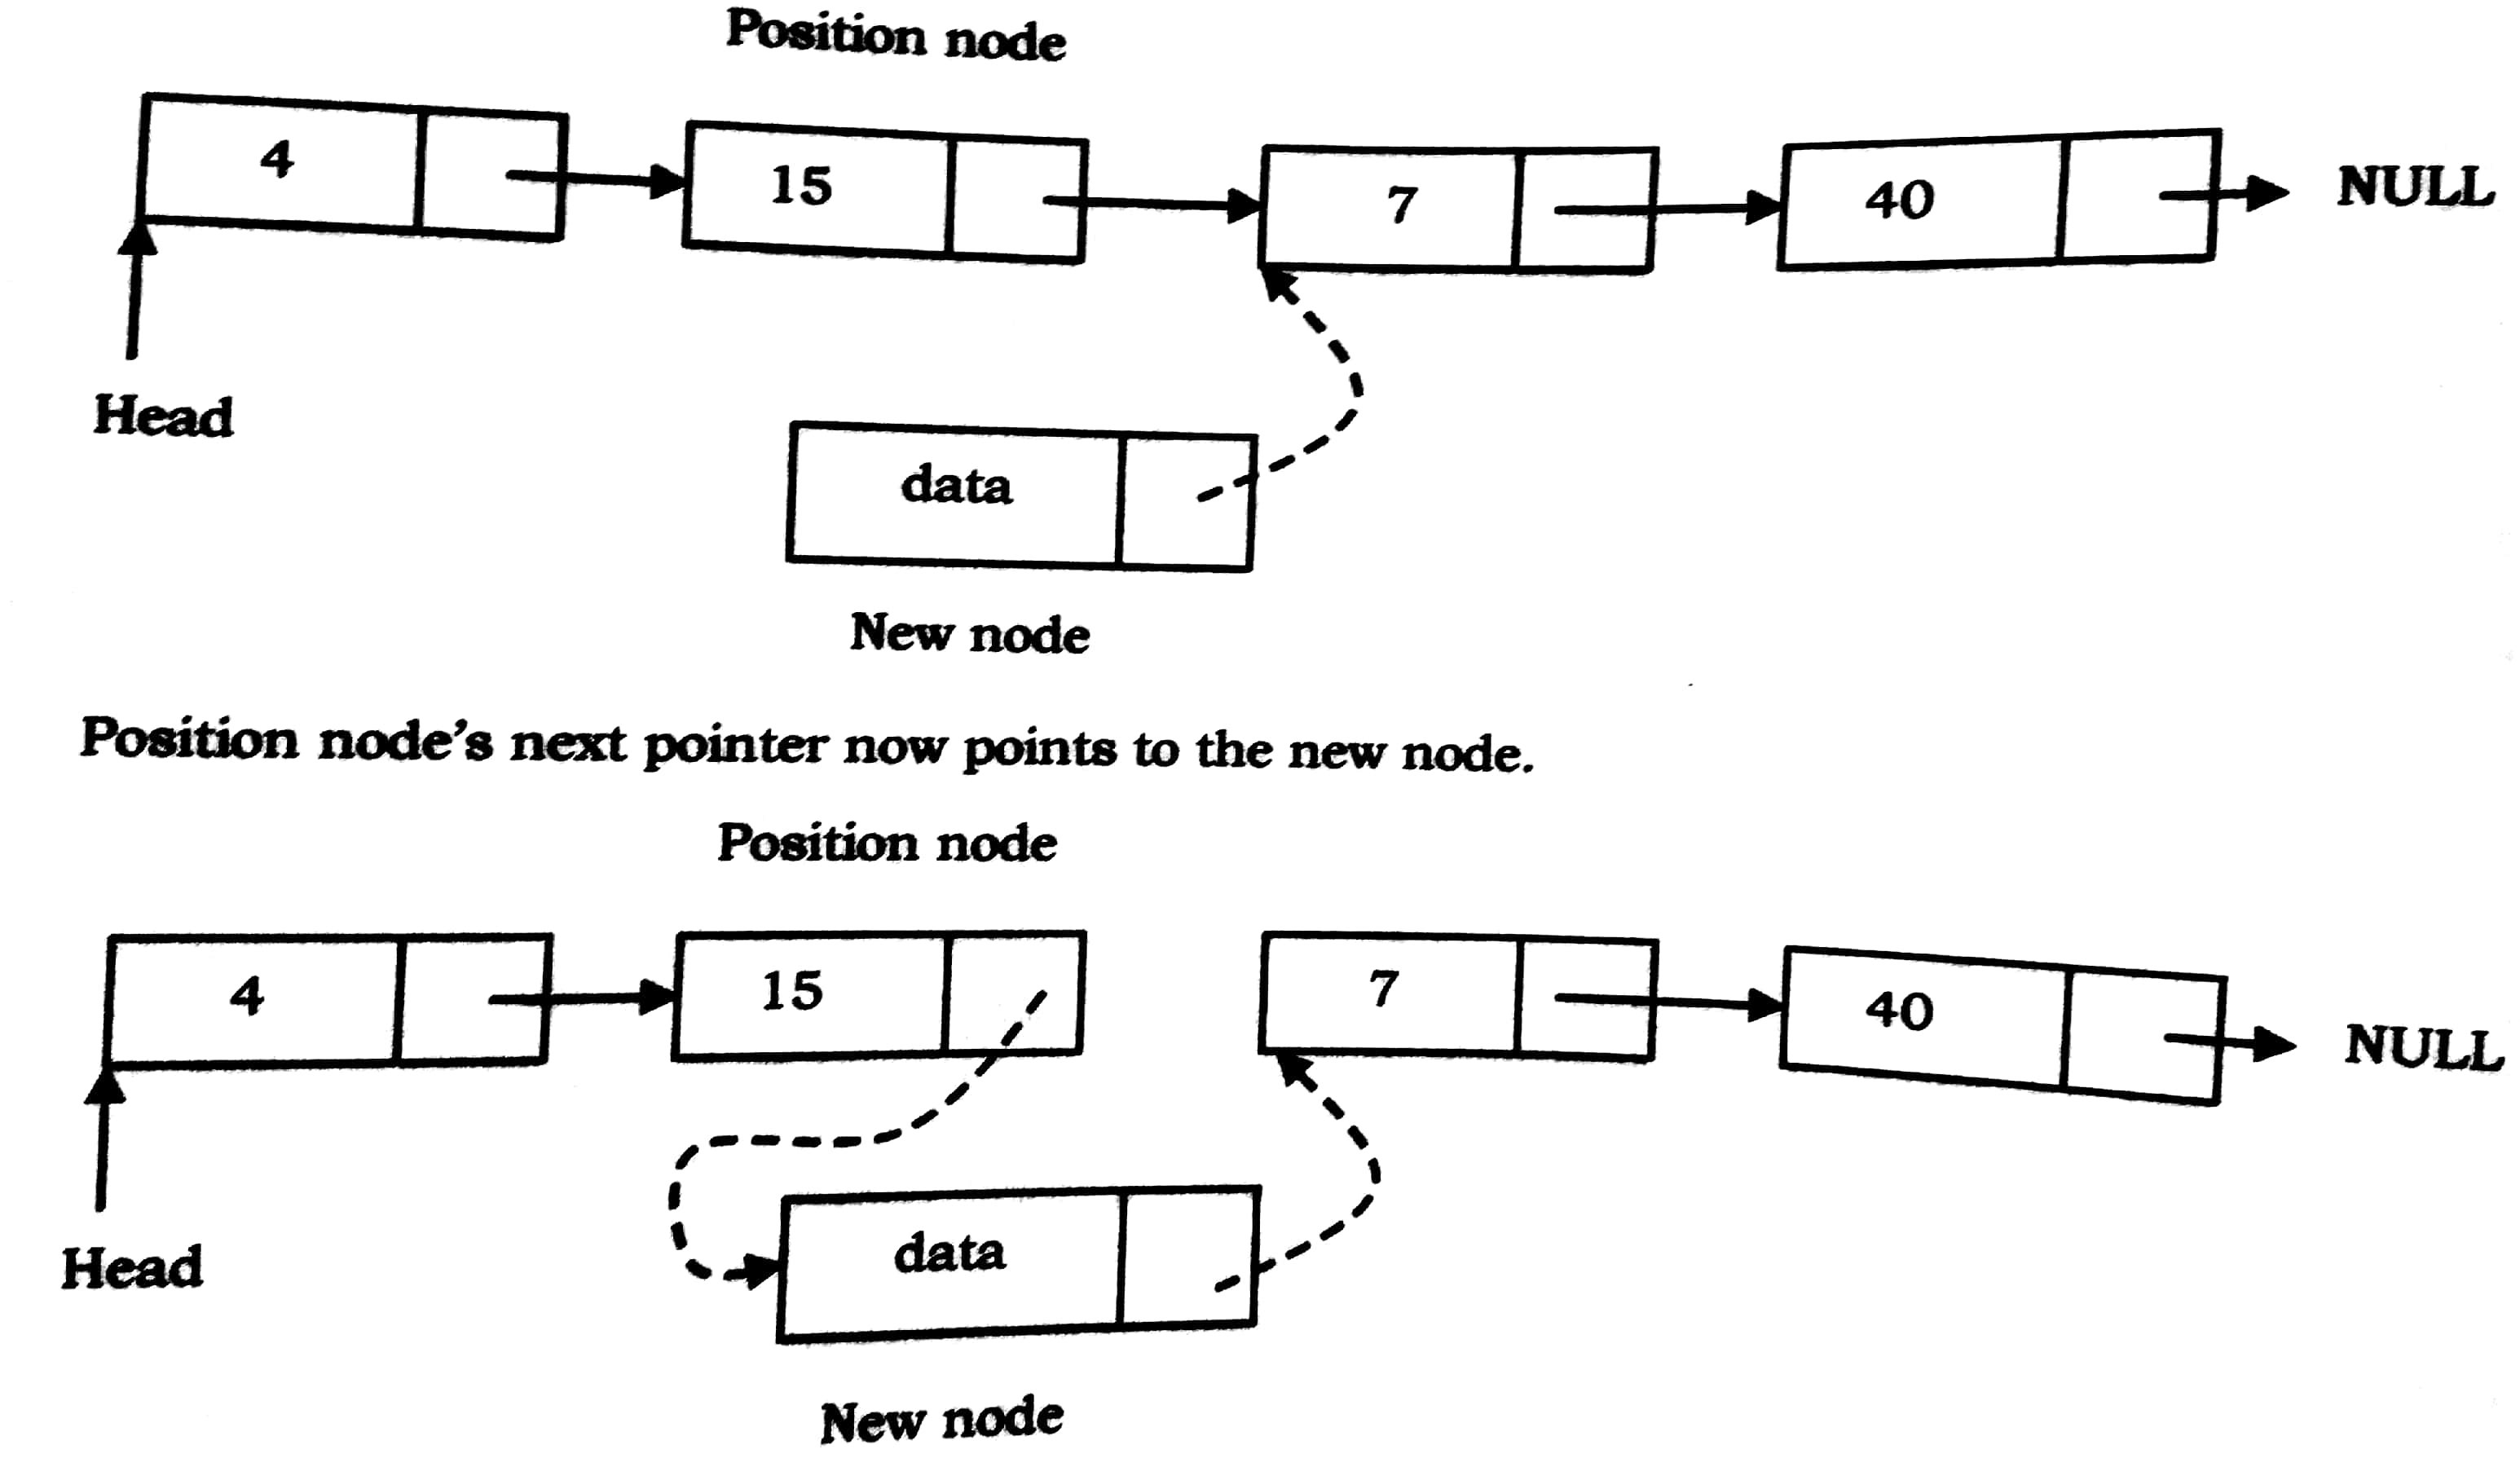
\includegraphics[scale=0.1]{figs/fig_listas/insere_posicao}
	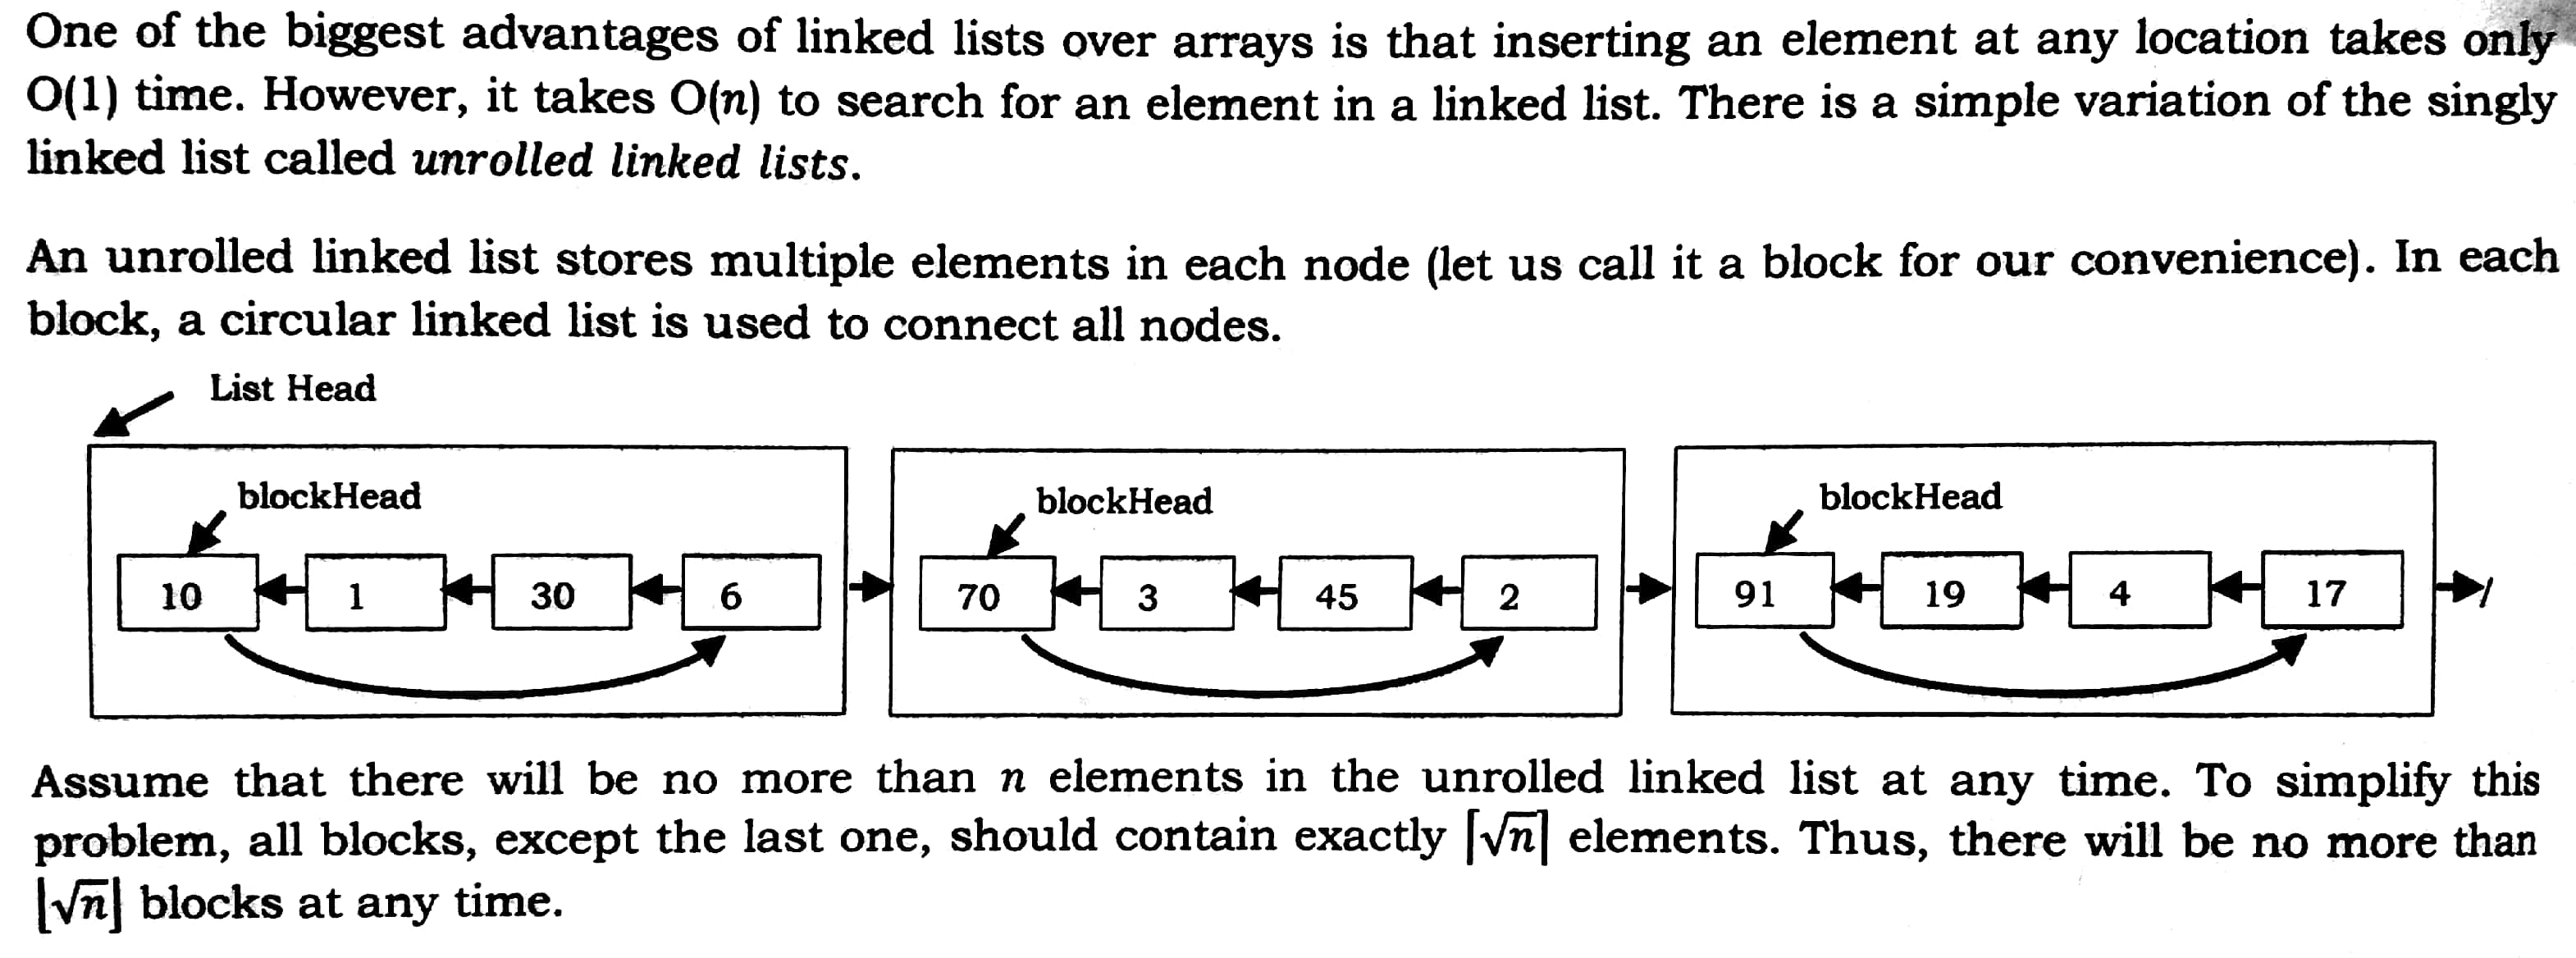
\includegraphics[height=0.60\paperheight, width=0.9\paperwidth]{figs/fig_listas/unrolled_listas.jpg}						
			\caption{Listas Encapsuladas}	
%%				\label{fig:lista-linear-repre}
		\end{figure} 

\end{frame} 

%ss------------------------------------------------------

\begin{frame}%%%[allowframebreaks=0.98]

\frametitle{Listas \textit{Niveladas} -- \textit{skiped}}

\begin{figure}[!hb]
	\centering
%%		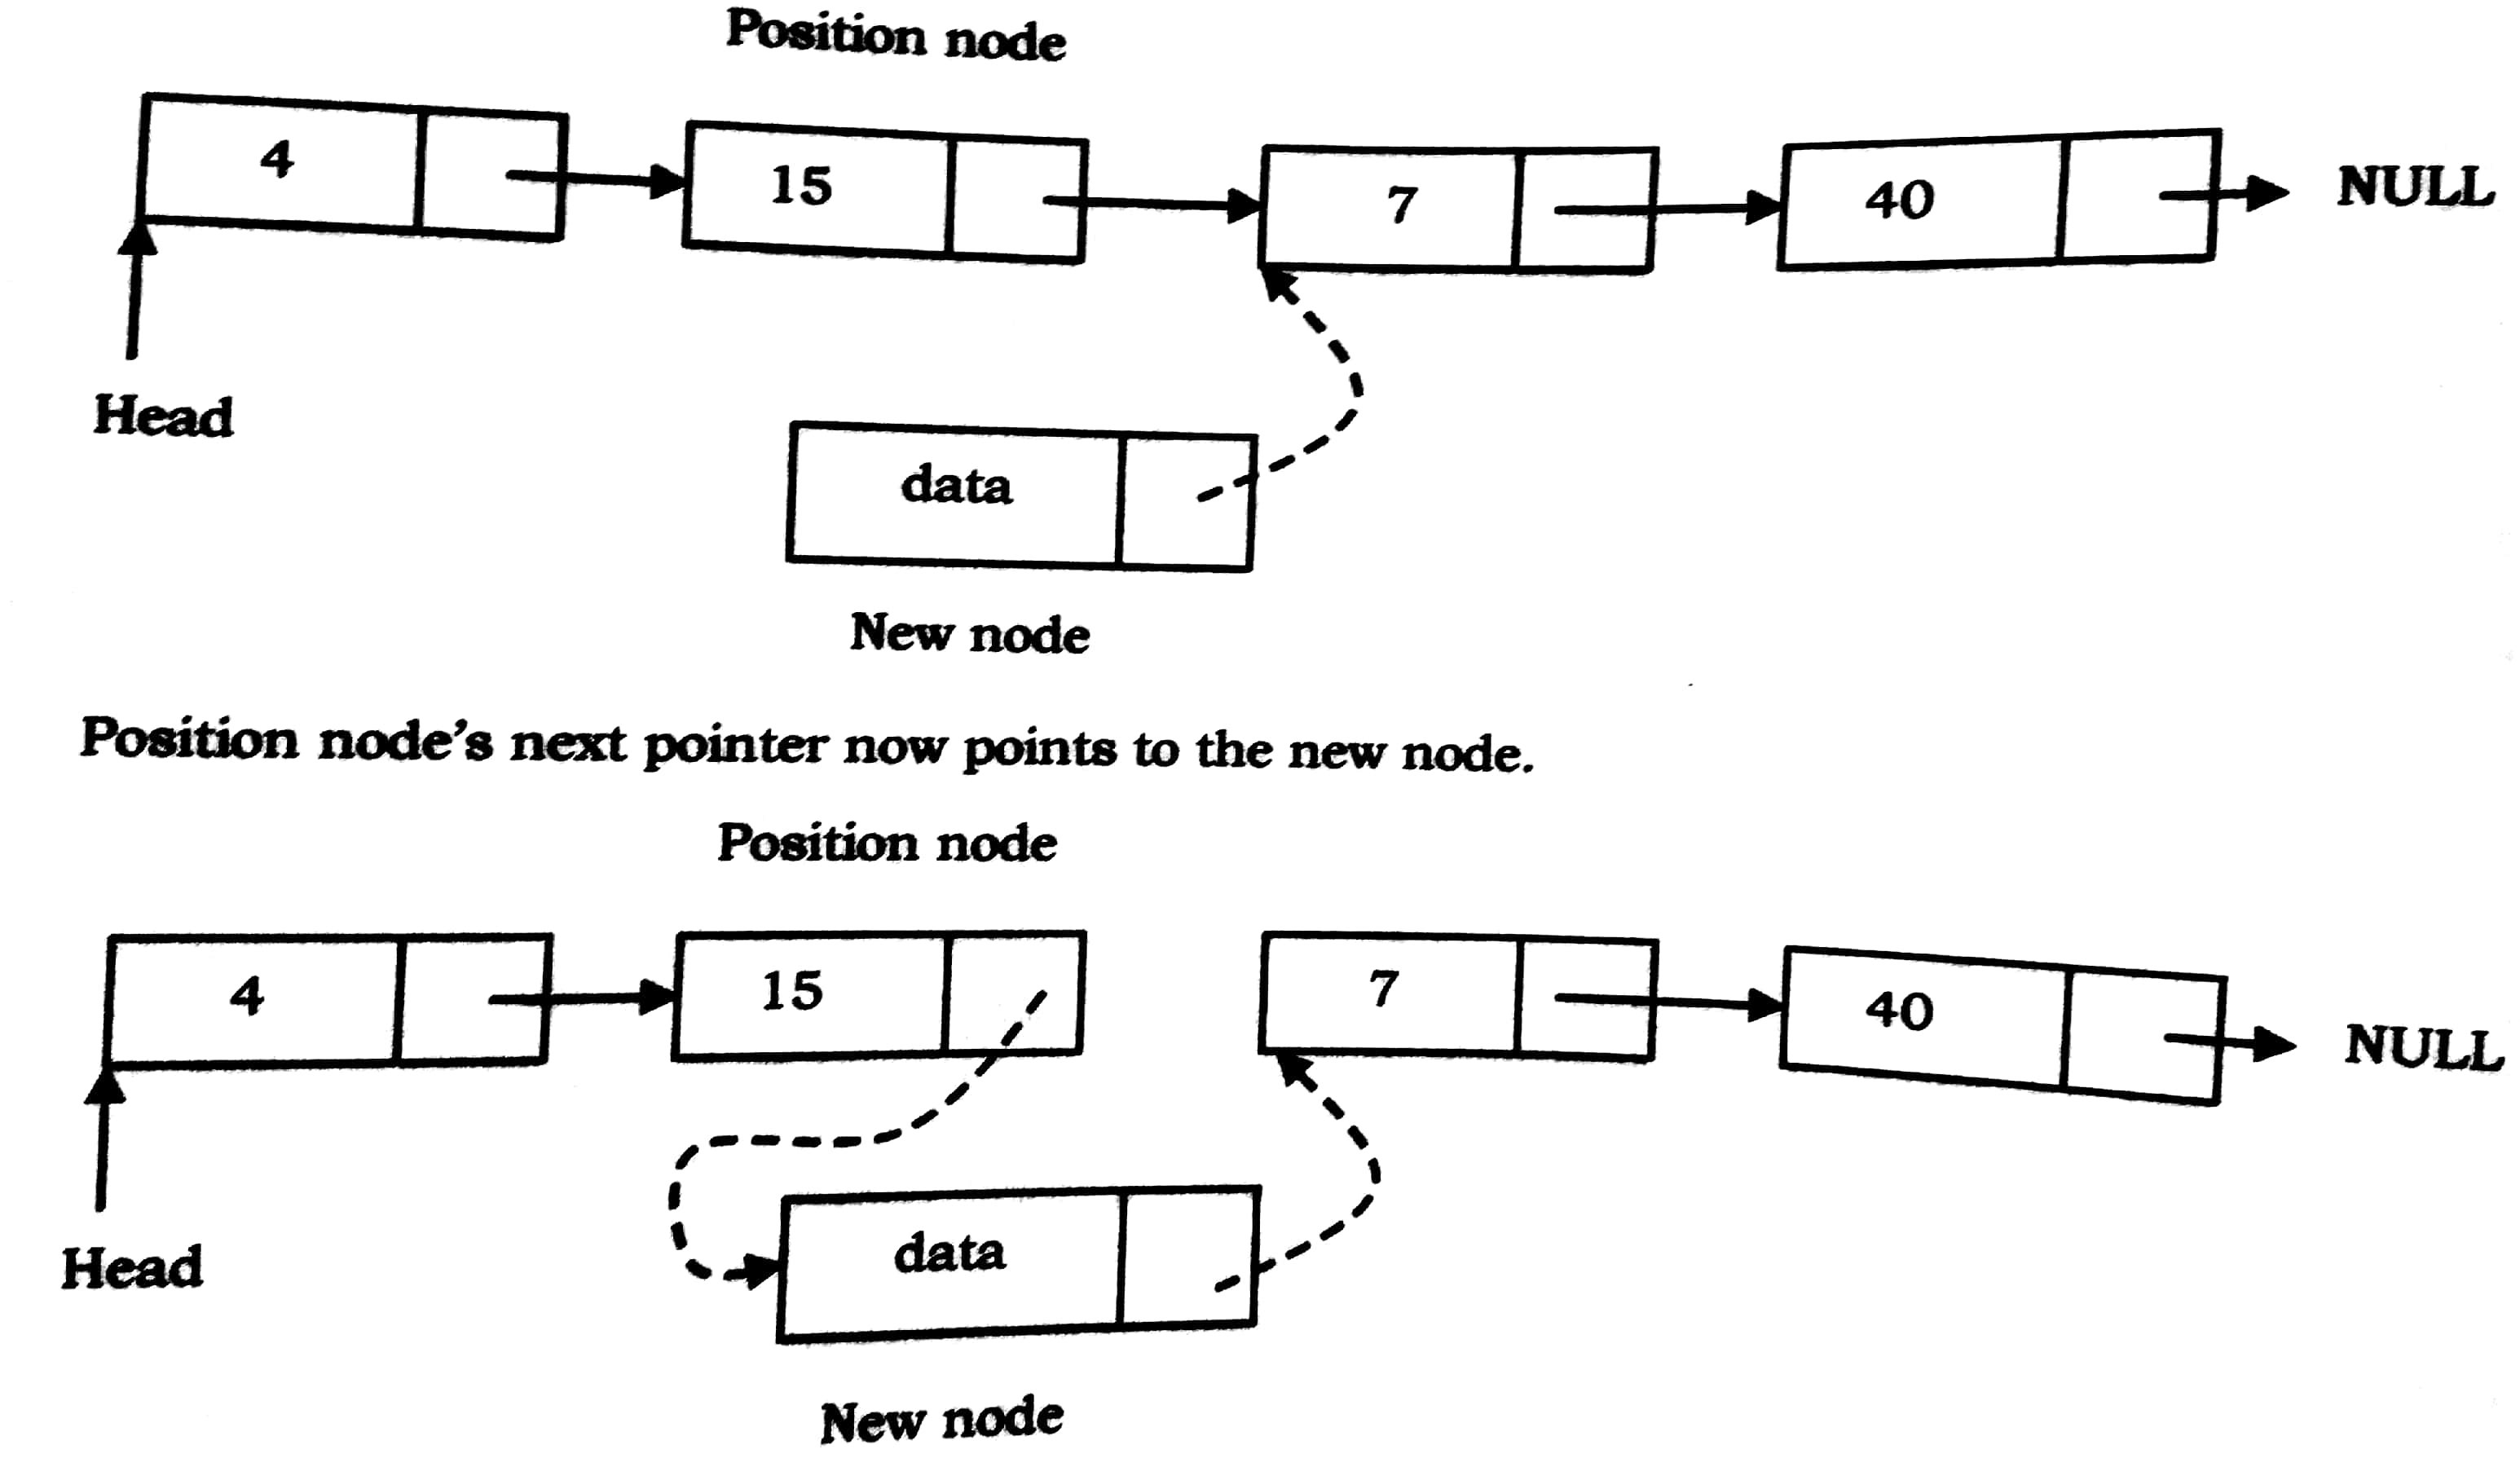
\includegraphics[scale=0.1]{figs/fig_listas/insere_posicao}
	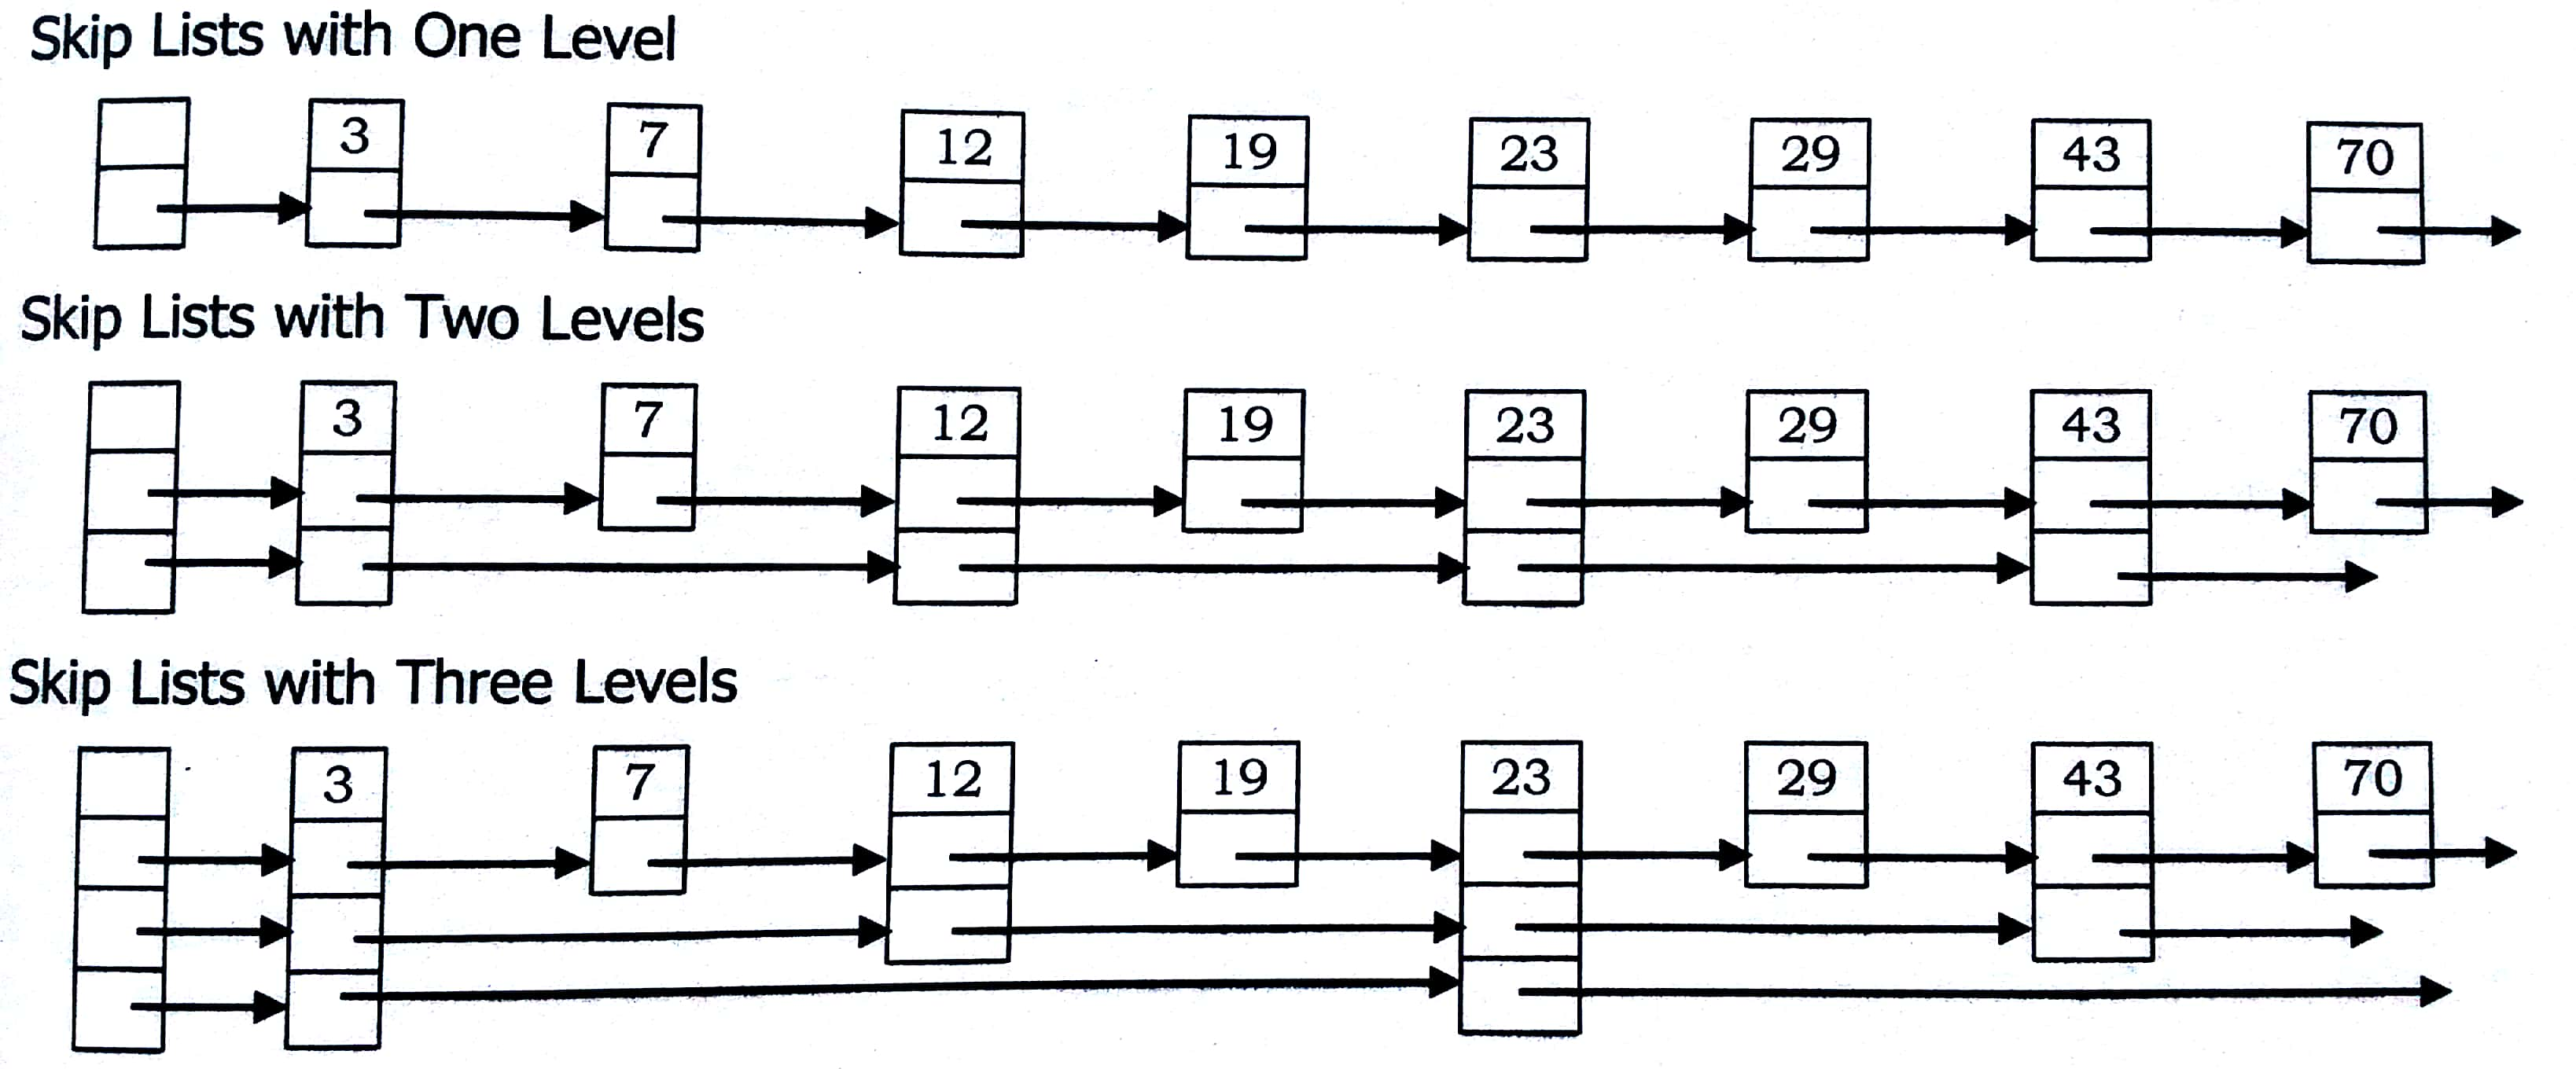
\includegraphics[height=0.50\paperheight, width=0.7\paperwidth]{figs/fig_listas/skipped_listas.jpg}						
			\caption{Listas Niveladas}	
%%				\label{fig:lista-linear-repre}
		\end{figure} 

\end{frame} 


\begin{frame}%%%[allowframebreaks=0.98]

\frametitle{Exercícios}

\begin{block}{Aqui esta \textit{lista} é grande ... }

\begin{itemize}
  \item Inverter a lista
  \item \textit{Merge} de duas listas
  \item Concatenar duas listas simples
  \item 
  \item 
  \item 
  
  
  
\end{itemize}


\end{block}


\end{frame} 

%%%%%%%%%%%------------------------------------------------------





\begin{frame}{Referências}
	\begin{enumerate}
	\item Karumanchi, Narashimha (2017). 
	\textit{Data Structures and Algorithms Made Easy -- Data Structures and Algorithms
		and Puzzles}.  CareerMonk.com

\item Tenenbaum, A. M., Langsam, Y., and Augestein, M. J. (1995). Estruturas de Dados Usando C. MAKRON Books, pp. 207-250.
\item Wirth, N. (1989). Algoritmos e Estrutura de dados. LTC, pp. 151-165.
	\end{enumerate}
\end{frame}
%----------------------------------------------------------------------------------------------------------
